\documentclass[a4paper,12pt]{article}

\usepackage[utf8]{inputenc}
\usepackage[french]{babel}
\usepackage[T1]{fontenc}
\usepackage{multirow,array}
\usepackage{graphicx}
\usepackage{a4wide}
\newcommand{\HRule}{\rule{\linewidth}{1mm}}

\begin{document}


%
%  TITRE
%

\begin{titlepage}

\begin{center}
\huge Une aide à la programmation sur GPU\\ pour le calcul scientifique
\HRule \\
\medskip
{\Huge \bfseries La librairie GMlib} \\
\HRule
\end{center}

\begin{figure}[htbp]
\begin{center}
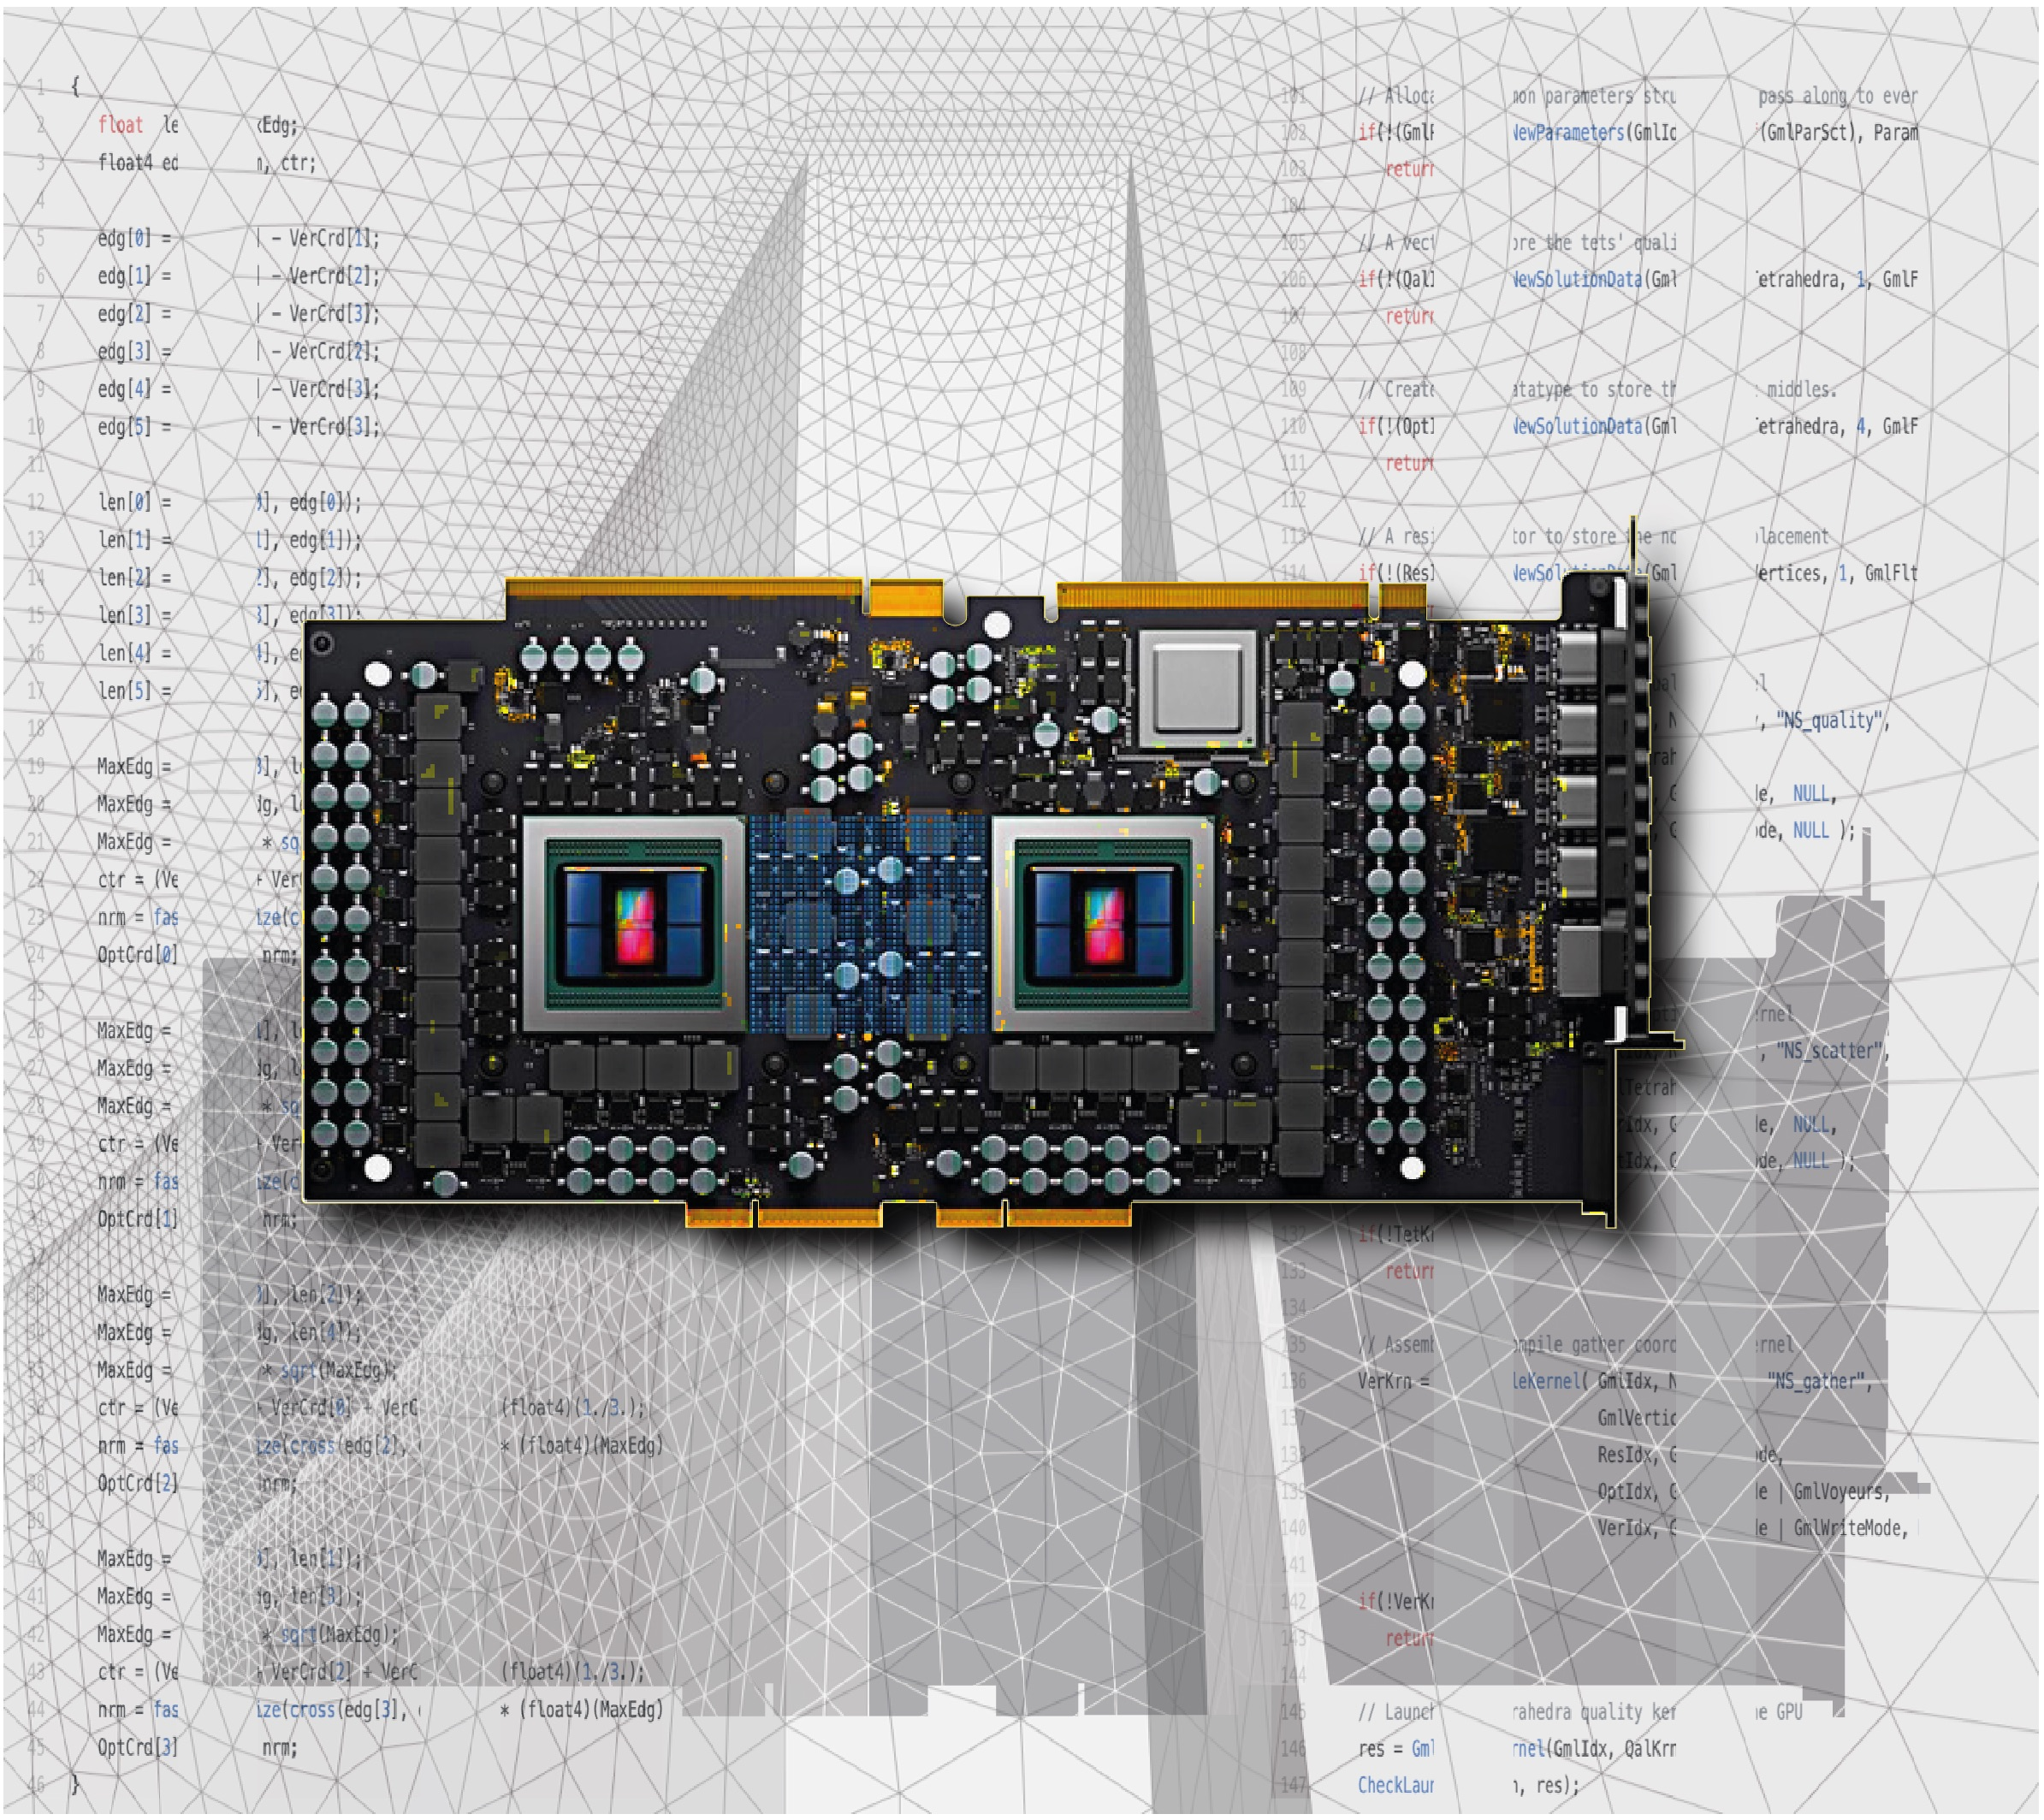
\includegraphics[width=15cm]{gpu.jpg}
\end{center}
\end{figure}

\begin{flushright}
\Large Lo\"ic MAR\'ECHAL / INRIA, Projet Gamma \\
\normalsize Juin 2020, document v2.08, librairie v3.29
\end{flushright}

\end{titlepage}

\clearpage

\setcounter{tocdepth}{2}
\tableofcontents
\vfill

\footnotesize{Couverture : création de Jean-Luc Maréchal.}
\normalsize

\clearpage


%
%  1 / INTRODUCTION
%


\section{Introduction}
La {\tt GMlib} v3 est une librairie visant à grandement faciliter le portage ou le développement sur GPU de logiciels de calculs scientifiques utilisant des maillages non structurés comme principale donnée.

Elle est basée sur le standard ouvert OpenCL, qui a pour avantage de fonctionner sur la plupart des matériels et systèmes actuels.
OpenCL fonctionne non seulement sur les GPU des trois principaux constructeurs, AMD, Intel et Nvidia, mais aussi sur les GPU intégrés des smartphones et tablettes (ARM, Imagination Technologies, etc.) et en l'absence de GPU dans un appareil, il est parfaitement à même d'utiliser efficacement tous les c\oe{}urs et capacités vectorielles des CPU, ce qui en fait une technologie très générique.

Mais le développement d'applications performantes et industrielles, c'est-à-dire, autre chose que la résolution d'un laplacien sur une grille structurée et carrée, requiert un investissement et des compétences conséquentes de la part du programmeur.
Il est donc important de préciser qu'en matière de programmation sur GPU, c'est le stockage, le transfert et l'accès efficace aux données qui sont le plus problématiques et non les algorithmes, qui ne nécessitent pas tant d'adaptation par rapport aux plateformes CPU parallèles conventionnelles.

C'est pourquoi l'idée sous-jacente de la {\tt GMlib} est d'abstraire autant que possible la gestion des données et de laisser le programmeur se concentrer le plus librement possible sur la partie algorithmique proprement dite.
Les GPU étant à l'origine conçus pour l'affichage graphique, il est naturel d'en utiliser le paradigme de programmation proposé par les principaux acteurs, connus sous le terme de \emph{shaders}.

L'approche du graphisme sur GPU consiste à demander au programmeur de transmettre l'ensemble des données nécessaires à l'affichage à la librairie graphique (OpenGL, Direct 3D ou Vulkan), puis de fournir un code assez succinct, appelé shader, à appliquer sur chacune des ces données graphiques.
Il est par exemple courant de fournir un ensemble de sommets, de vecteurs normaux associés et de triangles, et par la suite, de demander à la librairie graphique de boucler sur les triangles tout en accédant aux coordonnées et normales de leurs sommets afin d'exécuter un code (shader) calculant la couleur, l'ombrage et la position à l'écran de chaque pixel du triangle.

Une telle approche a été reprise par la {\tt GMlib}, mais ici les textures, projections, et effets graphiques sont remplacés par des tétraèdres, arêtes, champs de solutions physiques, et tous les accès indirects possibles entre ces entités.
Les types de données de maillage actuellement proposées sont : sommets, arêtes, triangles, quadrilatères, tétraèdres, pyramides, prismes et hexaèdres ainsi que les liens implicites qui les relient entre eux (boules, coquilles, voisins) et qui sont automatiquement construits par la librairie.

De plus, des types de données librement définissables (entier, flottant, scalaires, tableaux, vecteur) peuvent être associés à chaque entité de maillage afin d'y stocker les données nécessaires aux calculs.

Un code basé sur la {\tt GMlib} se déroule en quatre étapes : initialisations, renseignements des données, compilation des \emph{kernels} (nom donné aux \emph{shaders} dans le monde de la simulation numérique) et exécution de ces derniers sur GPU.

\paragraph{Initialisation :} on doit tout d'abord initialiser la librairie en lui fournissant le numéro du matériel qui va exécuter les kernels en OpenCL. Puis on dimensionne chaque type de donnée de maillage et de solution associée simplement en fournissant le nombre de chaque entité et la taille des données.

\paragraph{Renseignement des données :} l'utilisateur doit boucler sur chaque sommet, élément, ou autres données précédemment déclarés pour en transmettre le contenu à la {\tt GMlib}, qui elle-même se chargera de les transmettre sur la carte graphique au bon moment et sous une forme adéquate.

\paragraph{Compilation des kernels :} l'utilisateur décrit les boucles qu'il souhaite exécuter sur GPU en précisant pour chacune, la liste des entités de maillage et solutions qui lui seront nécessaires, ainsi que leur mode d'accès, lecture et/ou écriture, et enfin le code source du kernel à exécuter sur ces données et qui sera au préalable compilé par la librairie.
Cette compilation à chaud permet de générer un code binaire exécutable au moment même de l'exécution du logiciel et donc de fonctionner sur n'importe quel type de matériel (AMD, Intel, NVIDIA, etc.)

\paragraph{Exécution des kernels :} une fois toutes les données définies et transmises et les codes compilés et optimisés sur l'architecture choisie, il ne reste plus qu'a déclencher l'exécution de chaque kernel, autant de fois que nécessaire pour converger le calcul et en ne modifiant que quelques paramètres globaux afin de contrôler le processus numérique (coefficients, résidus, flags, etc.)


\subsection{Motivation}
Les deux principales motivations à la programmation sur GPU sont leur rapport performance/prix, bien plus intéressant que celui des CPU standards, ainsi que leur capacité d'évolution future, elle aussi bien plus grande que celle des CPU multic\oe urs qui semble être limitée à moyen terme.

Il faut néanmoins être réaliste, le prix d'une carte graphique haut de gamme est très élevé et souvent assez proche de celui d'un serveur de calcul. Quant aux performances annoncées par les constructeurs ou publiées dans de nombreux articles scientifiques surfant sur l'effet de mode des GPU, ils ne sont que théoriques. De nombreux codes d'exemples servant à démontrer la puissance des GPU n'utilisent que des algorithmes et des données simplifiées non représentatifs de la réalité industrielle de la simulation numérique. De plus, ils recourent à l'astuce de comparer un code sur GPU avec son équivalent séquentiel sur CPU... Les serveurs actuels possédant 12 ou 16 c\oe urs, la comparaison GPU / CPU multic\oe urs est nettement moins favorable.

Dans la pratique, le portage d'un code industriel travaillant sur des données réelles sur GPU ne saurait être plus de deux à quatre fois plus rapide qu'un bon serveur de calcul multi-c\oe urs. Ceci est déjà intéressant non seulement d'un point de vue prix, mais aussi d'encombrement (une carte d'extension contre plusieurs unités de racks) ou de consommation électrique.

Le gain espéré n'étant pas si extraordinaire, il est donc important pour un développeur de ne pas investir trop de temps dans une tentative de portage. Et c'est justement le problème de la programmation sur GPU : elle est très fastidieuse et consommatrice de temps !

Deux postes sont notamment lourds : la mise en forme et le transfert des structures de données de et vers le GPU, telles qu'elles soient assimilables et efficaces pour celui-ci, et le portage, l'optimisation et le débogage des algorithmes proprement dits dans le langage du GPU.

Il a donc paru important de proposer aux développeurs une librairie simplifiant ces deux aspects dans le cadre d'applications traitant des maillages, données de base de la plupart des codes de simulations numériques. La librairie proposée, la {\tt GMlib}, fournit donc au développeur des structures de données de maillages simples à définir et transférer ainsi qu'une panoplie de codes sources de base en OpenCL permettant d'y accéder efficacement.

Le mode opératoire est donc le suivant :

\begin{itemize}
\item choisir les types de données parmi ceux proposés qui vous permettront de stocker vos données,
\item partir d'un des codes de base proposés accédant à ce type de données et y insérer vos propres calculs sur ces données.
\end{itemize}

Ceci nous amène donc à parler de l'interfaçage entre vos données et la librairie, autrement dit, l'API.

\subsection{Installation et compilation}

La librairie est librement téléchargeable sur la page GitHub de l'auteur (cf. \cite{gmlib}) et le pacquage ZIP contient l'intégralité des sources, exemples et documentation.
Elle est mise à disposition sous la licence MIT (cf. \cite{MIT}) et peut donc être librement intégrée dans tout logiciel libre ou commercial, open ou closed source, inchangée ou modifiée, du moment que l'auteur est cité.

Le déploiement a été testé avec succès sous les systèmes \emph{Linux}, \emph{macOS} et \emph{Windows10}.
Sous macOS, l'environnement OpenCL fait partie intégrante du système et il n'est donc pas nécessaire d'installer quoique ce soit.
Ce n'est pas le cas des deux autres systèmes qui nécessitent d'installer un pilote adéquat, le plus souvent fourni par le fabricant de la carte graphique sur laquelle vous souhaitez exécuter les codes OpenCL.
Les trois principaux constructeurs, \emph{AMD}, \emph{Intel} et \emph{Nvidia}, proposent tous gratuitement des kits de développement GPU pour Linux et Windows10 dont les références sont ici : \cite{driver_amd}, \cite{driver_intel}, \cite{driver_nvidia}.

La {\tt GMlib} est composée du fichier C \emph{gmlib.c} et d'un header associé \emph{gmlib.h} et peut être simplement copié dans le répertoire source de votre projet pour y être recompilé et lié à la volée.
Dans ce cas, il est de la responsabilité de l'utilisateur de lier son exécutable avec la librairie OpenCL dont le nom et la localisation peuvent varier d'un système à l'autre.

C'est pourquoi un fichier \emph{cmakefile.txt} est fourni et permet une automatisation complète de la compilation et de l'installation de la librairie.
Il suffit d'exécuter {\tt cmake .} et {\tt make install} pour que la librairie, les utilitaires et exemples soient compilés et installés dans le répertoire /usr/local/bin par défaut.

La seule dépendance obligatoire est la librairie \emph{opencl} et il optionnellement, on peut aussi ajouter la {\tt libMeshb} afin d'ajouter des procédures d'import/export de fichiers \emph{.mshb} ou \emph{.solb} et de compiler les codes de démonstration.
Pour ce faire, il suffit de passer le paramètre de compilation {\tt -DWITH\_LIBMESHB} si vous compilez la librairie vous-même.
Le cmakefile quant à lui, détexte et ajouter automatiquement la {\tt libMeshb} si elle a elle aussi été installée via cmake.

Les fichiers installés sont les suivants :

\begin{itemize}
   \item la librairie statique gmlib.a
   \item le header gmlib.h
   \item la commande de transformation des sources OpenCl en header cl2h
   \item la documentation française GMlib\_fr.pdf
   \item plusieurs codes démonstration sous forme d'exécutables
   \item quelques fichiers de maillages utilisés par les démonstrations
\end{itemize}


%
%  2 / UTILISATION
%

\section{Utilisation}

\subsection{API}
\label{sec:API}
L'interaction avec la librairie repose sur deux éléments fondamentaux : les types de données et les codes (\emph{i. e.} kernels) qui vont opérer sur celles-ci. Par conséquent, le déroulement d'un logiciel utilisant un accélérateur GPU va se dérouler en deux phases :

\begin{itemize}
\item l'allocation et la définition des données, maillages, champs de solutions et liens topologiques,
\item la déclaration, la compilation et l'exécution des kernels en OpenCL.
\end{itemize}

Ces deux phases sont exécutées par le CPU hôte et seule les kernels tournent sur le GPU proprement dit et s'en trouveront donc accélérées. Dire d'un code qu'il "tourne sur GPU" est abus de langage, car les entrées-sorties, initialisations, compilations et post-traitements sont exécutés sur CPU et l'on devrait plutôt parler de logiciel hybride CPU/GPU ou bien accélérés par GPU. Il est donc important d'optimiser toutes les phases initiales sur CPU, car celle-ci représente le \emph{coefficient d'Amdahl} de tout code hybride CPU/GPU.

L'interfaçage avec la {\tt Gmlib} commence donc par son initialisation en lui fournissant le numéro du périphérique de calcul sur lequel tous les kernels seront exécutés : {\tt LibIdx = GmlInit(2);}

Sur la machine de l'auteur de ces lignes, une telle commande initialise la librairie avec la carte graphique \emph{ATI Radeon Pro 460} et l'étiquette retournée servira à communiquer avec toutes les autres commandes de la librairie par la suite.
Notez que plusieurs instances de la librairie peuvent être ouvertes simultanément, avec le même périphérique, ou bien un autre.

Remarque : une instance ne peut utiliser qu'un seul périphérique de calcul, composé lui-même de plusieurs \emph{compute units} et une seule zone mémoire, il s'agit donc de parallélisme à mémoire partagée.

Si l'utilisateur souhaite combiner la puissance de plusieurs GPU, il devra implémenter la distribution des calculs entre les cartes lui-même.

Il faut ensuite définir et renseigner les types de données qui seront utilisés par les calculs effectués sur le GPU. Cela introduit un aspect très important : l'utilisateur ne peut pas utiliser ses propres données en mémoire CPU (tableaux, structures, objets, etc.), mais doit obligatoirement les déclarer et les transférer à la librairie. C'est une contrainte très forte, car la nature des données offertes est assez limitée et le portage d'un code sur GPU va surtout consister à plier ses propres structures de données dans le canevas proposé par la {\tt GMlib}.

Pour illustrer le processus, on va déclarer et renseigner les sommets d'un maillage que l'on vient de lire, dans le tableau {\tt crd[n][3]} et assigner à chacun une vitesse et un vecteur de déplacement aléatoire.

\begin{tt}
\begin{verbatim}
VerIdx = GmlNewMeshData(LibIdx, GmlVertices, NmbVer);
for(i=0;i<NmbVer;i++)
   GmlSetDataLine(LibIdx, VerIdx, i, crd[i][0], crd[i][1], crd[i][2], 0);

VitIdx = GmlNewSolutionData(LibIdx, GmlVertices, 1, GmlFlt, "Vitesse");
for(i=0;i<NmbVer;i++)
{
   vitesse = rand();
   GmlSetDataLine(LibIdx, MasIdx, i, &vitesse);
}

DirIdx = GmlNewSolutionData(LibIdx, GmlVertices, 1, GmlFlt4, "Direction");
for(i=0;i<NmbVer;i++)
{
   vecteur[0] = rand();
   vecteur[1] = rand();
   vecteur[2] = rand();
   vecteur[3] = 0;
   GmlSetDataLine(LibIdx, MasIdx, i, &vecteur);
}
\end{verbatim}
\end{tt}
\normalfont

On souhaite calculer sur GPU le déplacement itératif de ces sommets selon leur direction et vitesse puis récupérer les coordonnées résultantes après 1000 itérations.

Pour cela, nous allons tout d'abord écrire le code de déplacement d'une itération en OpenCL : il s'agit d'un kernel et il doit être placé dans un fichier indépendant, que nous appellerons \emph{iteration.cl}.

Puis on va le compiler en lui passant en paramètres les données préalablement définies : les sommets qu'on souhaite envoyer sur le GPU et récupérer à la fin (\emph{Read \& Write}) et la vitesse et le déplacement qu'on souhaite seulement envoyer, mais pas récupérer (\emph{Read}).

\begin{tt}
\begin{verbatim}
KrnIdx = GmlCompileKernel( LibIdx,  iteration, "iteration", GmlVertices, 3,
                           VerIdx, GmlReadMode | GmlWriteMode, NULL,
                           VitIdx, GmlReadMode               , NULL,
                           DirIdx, GmlReadMode               , NULL );
\end{verbatim}
\end{tt}
\normalfont

Et voici le fameux kernel nommé \emph{iteration.cl} : 

\begin{tt}
\begin{verbatim}
VerCrd = VerCrd + VerVitesse * VerDirection;
\end{verbatim}
\end{tt}
\normalfont

Ce code, on ne peut plus succinct, amène de nombreuses remarques :

\begin{itemize}
\item il n'y a pas de boucle itérant de 1 à NmbVer,
\item il ne comporte aucune définition préalable des variables utilisées,
\item il n'y a pas d'accès aux tableaux des sommets et données associées, mais seulement des scalaires préremplis,
\item on ne sait pas comment sera stocké le résultat,
\item les coordonnées et le champ de déplacement sont des vecteurs en 3-D.
\end{itemize}

\paragraph{Boucle implicite : } il y a bien un compteur de boucle qui est incrémenté de 1 à NmbVer, mais la boucle est effectué par le GPU et l'utilisateur n'a pas moyen de contrôler l'ordre de traitement des sommets.
Il ne fournit que le noyau de la boucle (d'où le nom \emph{kernel}), sans itérateur, et ce morceau de code sera instancié et exécuté autant de fois qu'il y a de sommets dans le maillage, mais dans un ordre non spécifié.

\paragraph{Variables implicites : } les déclarations de variables locales sont effectuées par la librairie en fonction des paramètres définis lors de la compilation du kernel.
Comme nous avons demandé l'accès aux coordonnées des sommets (un vecteur 3-D), à la vitesse (un scalaire) et au vecteur de déplacement (un vecteur 3-D), la librairie a donc défini d'elle-même les variables du type adéquat pour recevoir toutes les données demandées associées à l'unique sommet en cours de traitement.

Les noms des données de type maillage sont imposés par la librairie et connus (VerCrd pour les coordonnées, TriVer pour les numéros des trois sommets d'un triangle, etc.), quant aux données librement définies par l'utilisateur, elles portent le nom qu'il leur a assigné au moment de l'initialisation.

Dans notre exemple, {\tt vitesse} est un scalaire et {\tt direction} est un vecteur. Le code OpenCL des définitions est en fait créé par la librairie et ajouté juste avant le kernel fourni par l'utilisateur.

\paragraph{Accès aux tableaux globaux : } il n'y a pas qu'un seul sommet dans le maillage et pourtant la librairie n'a défini qu'un seul vecteur {\tt VerCrd} contentant les coordonnées d'un seul sommet.
Là encore, la librairie a bien défini le tableau des coordonnées ({\tt VerCrdTab[ NmbVer ]}), mais celui-ci est caché à l'utilisateur et les coordonnées du sommet en cours de traitement sont automatiquement lues avant de passer la main au kernel.

De fait, lorsque l'unique ligne du kernel d'exemple commence à être exécutée, la librairie a déjà rempli les variables locales avec les données du sommet courant \emph{i} : {\tt VerCrd = VerCrdTab[i]}, {\tt vitesse = vitesseTab[i]}, {\tt direction = directionTab[i]} et il n'a pas à se soucier du transfert des variables globales vers les locales sur lesquelles les calculs seront effectués.

\paragraph{Stockage du résultat en mémoire : } de la même manière qu'avec les lectures, toutes les variables étant définies comme \emph{Write} au moment de la compilation seront stockées dans les tableaux globaux après l'exécution du kernel utilisateur.
Cette écriture est cachée et transparente. Dans l'exemple, seules les coordonnées sont accédées en écriture et la librairie rajoutera d'elle-même la ligne suivante : {\tt VerCrdTab[i] = VerCrd} afin de stocker le résultat du calcul sur ce sommet dans la mémoire du GPU, d'éventuels calculs intermédiaires seront perdus !

\paragraph{Calcul vectoriel : } le langage OpenCL offre des variantes scalaires et vectorielles de tailles 2, 4, 8 ou 16 pour chaque type de données entières (codées sur 8, 16, 32 ou 64 bits) et réelles (16, 32 ou 64 bits) et utilise la technique du surtypage d'opérateur pour adapter les opérations aux types des opérandes.

Dans notre kernel, {\tt VerCrd} et {\tt direction} sont des vecteurs 3-D et effectuer l'opération {\tt VerCrd = VerCrd + direction} va déclencher une addition vectorielle traitant les trois coordonnées simultanément.

Que se passe-t-il alors lorsqu'on multiplie le déplacement par le scalaire contenant la vitesse ?

Le compilateur détecte la différence de type et choisit l'opération appropriée, dans le cas présent, il va utiliser la fonction multipliant tous les termes d'un vecteur par un scalaire.


\subsection{Les types de données}

L'utilisateur étant contraint à utiliser uniquement les types de données proposés, il est donc très important de bien en comprendre le fonctionnement et tous les usages possibles.
Ces types se regroupent en trois catégories : les données des maillages (sommets, arêtes, triangles, etc.), les champs de solutions libres (des tableaux, scalaires ou vecteurs associés à chaque entité d'un type de maillage) et enfin les liens topologiques, de loin les plus complexes, qui permettent des accès indirects efficaces entres tous les différents types (boules des points, voisinages par face, coquille d'arêtes, etc.).

\paragraph{Types de données de maillage :} ils permettent de représenter tout maillage hybride à l'ordre un, les ordres deux et trois étant prévus pour une version ultérieure.
Sont donc proposés les types classiques, Vertices, Edges, Triangles, Quadrilaterals, Tetrahedra, Pyramids, Prisms et Hexahedra.

Les sommets (Vertices) sont composés de trois flottants et d'un entier pour stocker les coordonnées et la référence physique, et tous les autres éléments sont composés de 2 à 8 entiers pour stocker les numéros de sommets ainsi qu'un entier supplémentaire pour la référence.

Remarque : tous les indices de tableaux vont de $0$ à $n-1$.

Leur allocation se fait avec la commande {\tt GmlNewMeshData}, en spécifiant simplement le nombre d'entités souhaitées dans le maillage.

Notez qu'une instance de la librairie ne peut comporter qu'un seul tableau d'un même type de maillage, il n'est donc pas possible d'allouer deux tableaux de triangles par exemple.

Leur renseignement se fait ensuite avec la commande {\tt GmlSetDataLine}, en précisant le type de la donnée, le numéro de l'entité (de 0 à n-1), puis un nombre variable d'arguments correspondant aux données composant l'élément en question.
L'exemple suivant alloue et renseigne trois sommets :

\begin{tt}
\begin{verbatim}
VerIdx = GmlNewMeshData(LibIdx, GmlVertices, 3);
GmlSetDataLine(LibIdx, VerIdx, 0, 1.5, 2.3, 1.0, 8);
GmlSetDataLine(LibIdx, VerIdx, 1, 9.2, 8.3, 1.0, 6);
GmlSetDataLine(LibIdx, VerIdx, 2, 6.3, 1.6, 2.3, 0);
\end{verbatim}
\end{tt}
\normalfont

\paragraph{Les champs associés : } ils permettent d'associer des données librement à toutes les entités d'un type de maillage donné.
Il ne peut y avoir qu'un seul type de donnée OpenCL dans un champ, mais ce type peut être vectoriel (taille de 2 à 16) et peut même être composé d'un tableau de vecteurs.
Les types scalaires proposés sont : \emph{byte}, \emph{int}, \emph{float} et \emph{double} ainsi que leurs déclinaisons vectorielles.
Chaque type de solution est associé à un type de maillage précis, mais il est possible de déclarer autant de champs associés pour chaque type de donnée de maillage que nécessaire ce qui permet de simuler l’équivalent d'une structure hybride, chaque champ stockant un type OpenCL différent.

L'allocation se fait avec la commande {\tt GmlNewSolutionData}, en spécifiant le type de maillage auquel ce champ de solution est associé, la taille du tableau local associé à une entité de maillage (= 1 pour un scalaire), ainsi que le type de la donnée (GmlByte, GmlInt16, GmlFloat4, etc.) et le nom sous lequel apparaitra la variable déclarée automatiquement.
Les données sont renseignées avec la commande {\tt GmlSetDataLine}, mais contrairement aux éléments, on ne passe pas toutes les valeurs des champs explicitement, mais seulement un pointeur sur un tableau contenant la totalité du champ associé à cette entité et qui sera recopié dans la structure interne de la librairie.

L'exemple suivant alloue et renseigne un tableau de deux flottants pour chacun des trois sommets alloués précédemment :

\begin{tt}
\begin{verbatim}
float vec[2];
VecIdx = GmlNewSolutionData(LibIdx, GmlVertices, 2, GmlFlt, "masse_vitesse");
vec = {1.2, -6.3};
GmlSetDataLine(LibIdx, VecIdx, 0, &vec);
vec = {0.3,  5.2};
GmlSetDataLine(LibIdx, VecIdx, 1, &vec);
vec = {3.4, -0.1};
GmlSetDataLine(LibIdx, VecIdx, 2, &vec);
\end{verbatim}
\end{tt}
\normalfont

\paragraph{Les liens topologiques : } c'est l'entité la plus complexe à appréhender et manipuler, mais aussi la plus puissante, grâce à elle, et un peu d'imagination, on peut contourner l'essentiel des limitations imposées par le calcul sur GPU.
Un lien topologique permet de lier un type de maillage source et un type de destination, par exemple lier les triangles vers les tétraèdres, ce qui consiste à fournir les indices des deux tétraèdres voisins pour chaque triangle.
Un tel tableau serait associé aux triangles (la source) et serait composé de deux entiers par triangles, car un maximum de deux tétraèdres peut partager un même triangle.

Les liens ne sont pas commutatifs, car inverser les triangles et les tétraèdres revient à donner pour chaque tétraèdre (la source), la liste des quatre triangles qui constituent ses faces.
Ces liens topologiques vont être utilisés dans les kernels à accès mémoire indirect, voir section \ref{sec:kernels_indirects}, et permettront d'accéder aux données associées aux tétraèdres dans une boucle sur les triangles, pour reprendre notre premier exemple.

Un des points forts de la {\tt GMlib} est qu'elle va automatiquement construire les liens standards entre tous les types de données, et ce au moment de la compilation d'un kernel.

Par exemple, si on demande une boucle sur les arêtes, et que des données à lires sont associées à des triangles, la coquille des triangles pour chaque arête sera construite.
L'utilisateur ne sera amené à créer ses propres liens topologiques que pour effectuer des accès mémoires indirects spécifiques à son algorithme, par exemple, donner les deux triangles \emph{upwind} et \emph{downwind} pour chaque arête dans un solveur fluide.

Dans un tel cas en 2-D, si l'utilisateur demandait une boucle sur les arêtes et voulait lire des données de calculs associées aux triangles, la librairie construirait le lien topologique naturel partant des arêtes pour pointer sur les triangles : il s'agirait donc des deux triangles partageant une même arête, et ce n'est pas ce dont le solveur a besoin.
Dans ce cas, il sera de la responsabilité de l'utilisateur d'allouer un type de donnée topologique avec la commande {\tt GmlNewLinkData} en précisant les étiquettes des types source et destination ainsi que le nombre de liens nécessaires pour chaque source.
Vous pourriez, pourquoi pas, avoir envie de créer une table donnant pour chaque sommet les indices des 180 pyramides les plus proches !

L'allocation et le remplissage sont similaires aux champs associés :

\begin{tt}
\begin{verbatim}
int pyramides[ NmbVer ][ 180 ];
PyrIdx = GmlNewLinkData(LibIdx, GmlVertices, GmlPyramides, 180, "Gizeh");
for(i=0;i<NmbVer;i++)
   GmlSetDataLine(LibIdx, PyrIdx, pyramides[i]);
\end{verbatim}
\end{tt}
\normalfont

Remarque : le lien inverse de sommet vers pyramides, soit une pyramide vers ses cinq sommets, n'est rien d'autre que le tableau des éléments pyramidaux lui-même.
De fait, tous les éléments du maillage ne sont que des liens entre de un numéro d'élément et plusieurs numéros de sommets.

\subsection{Kernels à accès directs}
\label{sec:kernels_directs}
C'est le type de Kernel le plus simple et comme tout kernel il ne boucle que sur les éléments d'un seul type, et n'accède en lecture ou en écriture qu'à des données relatives au type d'élément de la boucle.

Si on boucle sur les sommets et accède à un champ de solution qui leur est associé, tous les tableaux seront accédés via l'indice de boucle principal : il n'y a donc aucune indirection mémoire.
C'est aussi le type de Kernel le plus efficace, car il utilise à 100\% la bande passante de la mémoire du GPU étant donné que les tableaux sont lus linéairement.

Dans l'exemple introductif de la section \ref{sec:API}, les deux types de solutions alloués sont relatifs aux sommets et le kernel d'une ligne boucle sur ces sommets et accède aux coordonnées en lecture et écriture et aux solutions en lecture seulement.

\begin{tt}
\begin{verbatim}
VerCrd = VerCrd + VerVitesse * VerDirection;
\end{verbatim}
\end{tt}
\normalfont

Dans ce kernel, à chaque itération de la boucle de 0 à NmbVer, les coordonnées, la vitesse et le vecteur de direction sont tous lus de manière cachée par la librairie qui y accède via l'indice de boucle principal $i$.
Dans les faits, un GPU transférant tout d'abord la mémoire par blocs de 32 ou 64 entiers consécutifs vers la mémoire cache et accédant ensuite à cette dernière, l'accès à la case {\tt vitesse[0]} va déclencher la lecture de {\tt vitesse[0..31]}, puis les accès suivants, de 1 à 31, ne couteront que le prix d'un accès au cache.

Dans cette configuration, le nommage des variables automatique est évident, elles portent le nom court du type de maillage de la boucle principale auquel est concaténé le nom de la variable accédée.
Dans notre exemple, la boucle portant sur les {\tt GmlVertices} (nom court {\tt Ver}), et on accède aux coordonnées ({\tt Crd}), à la vitesse ({\tt Vitesse}) et au vecteur de direction ({\tt Direction}), ce qui donne les noms automatiques suivants : {\tt VerCrd}, {\tt VerVitesse} et {\tt VerDirection}, élémentaire !

Remarque : les accès directs aux données peuvent être fait en mode lecture, ou écriture, ou bien les deux en même temps.

\subsection{Kernels a accès indirects}
\label{sec:kernels_indirects}
C'est ici que les choses deviennent un peu plus sérieuses.
Un kernel est dit à accès indirect lorsqu'il est amené à lire des données associées à un type de maillage différent de celui de la boucle principale.
Dans un tel cas, les accès mémoires prennent la forme {\tt a = u[v[i]]} et non plus {\tt a = u[i]} comme c'est le cas dans les accès directs.

Ces accès indirects sont nettement plus lents pour deux raisons.

Tout d'abord il faut effectuer deux accès mémoire pour obtenir une seule valeur utile au final.
Le GPU commence par déclencher une première lecture {\tt tmp = v[i]}, puis lit {\tt a = u[ tmp ]}.

Enfin et surtout, les accès successifs à {\tt a = u[ tmp ]} ne sont pas consécutifs en mémoire lorsqu'on incrémente le compteur, $i$ car les valeurs contenues dans {\tt v[i]} sont totalement inconnues au moment de la compilation et dépendent uniquement de la numérotation des éléments et sommets du maillage.

Afin de limiter le problème, on recourt à deux méthodes, la renumérotation du maillage par une courbe de Hilbert (ou toute autre SFC) afin d'améliorer l'efficacité de la mémoire cache, ainsi qu'a la vectorisation des liens montants (boules de points, coquilles d'arêtes), par nature irréguliers, pour en améliorer la compacité d'accès mémoire (cf. \cite{peano_hilbert}).
Le déroulement de ces kernels est totalement transparent pour l'utilisateur, car la librairie va se charger de lire le tableau d'indirection, puis les données ainsi accédées.
Dans le cas d'une boucle sur les triangles ({\tt Tri}), si on souhaite accéder aux coordonnées des sommets ({\tt Crd}), la librairie va d'elle-même définir et remplir un tableau ({\tt TriVer[3]}) de trois vecteurs contenant les coordonnées des trois sommets du triangle.

À titre d'illustration, voici un code bouclant sur les triangles et calculant leur barycentre :

\begin{tt}
\begin{verbatim}
KrnIdx = GmlCompileKernel( LibIdx,  barycentre, "barycentre", GmlTriangles, 3,
                           VerIdx, GmlReadMode , NULL,
                           TriIdx, GmlReadMode , NULL,
                           BarIdx, GmlWriteMode, NULL );
\end{verbatim}
\end{tt}
\normalfont

Et voici le kernel indirect associé :

\begin{tt}
\begin{verbatim}
Bar = (TriCrd[0] + TriCrd[1] + TriCrd[3]) / 3.;
\end{verbatim}
\end{tt}
\normalfont

La variable {\tt Bar} est un unique vecteur de coordonnées, car il est relatif au triangle qui est l'élément de la boucle principal, alors que la variable {\tt TriCrd} est un tableau de taille 3, car elle est relative aux sommets d'un triangle qui en compte trois.

Comme vous pouvez le constater, il n'est nul besoin d'accéder explicitement aux numéros des trois sommets du triangle, ceci étant effectué par la librairie juste avant de passer la main au kernel de l'utilisateur.
Un lien topologique est donc une structure complètement muette et transparente.
Ce qui peut être perturbant, c'est que différentes commandes de compilation d'un même kernel mais avec {\tt GmlEdges} à la place de {\tt GmlTriangles} par exemple, va produire des codes différents !
En effet, la variable contenant les coordonnées s'appellera alors {\tt EdgCrd[2]} et sa taille sera de deux au lieu de trois dans le cas d'une boucle principale sur les triangles.
On parle alors de variable et de programmation contextuelle.

Une fois maitrisé ce concept, il est alors possible d'accéder indirectement (en lecture seulement) à n'importe quel type de données (maillage ou solution) associées à des types de maillage complètement différents du type de la boucle principale, car tous les cas possibles de liens indirects sont gérés par automatiquement par la {\tt GMlib}.

\paragraph{Liens topologiques descendants, transverses et montants :} un lien est descendant si le type de la boucle est de dimension strictement supérieure au type accédé indirectement (exemple : triangle vers arêtes), transverse si les deux types sont de même dimension (triangle vers les triangles ou quadrilatères voisins) et montant si la dimension du type indirect est strictement supérieure au type de la boucle (boucle sur les sommets et accès aux triangles de leurs boules).

\paragraph{Lien descendant :} ce premier type est trivial, il s'agit le plus souvent de boucler sur un élément et d'accéder aux données associées à ses sommets.
Dans ce cas, la table d'indirection est la liste des noeuds composant chaque élément et la librairie n'a qu'à la transmettre telle quelle au GPU.

\paragraph{Lien transverse :} le second type, présente une petite finesse, car par défaut, si on boucle sur les triangles et qu'on accède à des données relatives à chaque triangle, il s'agit tout simplement d'un accès direct comme vu à la section \ref{sec:kernels_directs}.
Mais il est aussi possible de fournir un tableau de liens topologiques spécifiques au moment de la compilation du kernel, comme un tableau des voisins par arêtes.
Dans ce cas, on pourra boucler sur les triangles et accéder à des données relatives au triangle en cours de traitement ainsi qu'à ses trois voisins.
Le code suivant va récupérer les barycentres des triangles, calculés à l'exemple précédent, en même temps que ceux de leurs trois voisins, afin de déterminer la distance maximum entre le centre d'un triangle et celui de ses voisins.

\begin{tt}
\begin{verbatim}
NgbIdx = GmlSetNeighbours(LibIdx, GmlTriangles);
DisIdx = GmlNewSolutionData(LibIdx, GmlTriangles, 1, GmlFlt, "distance");
KrnIdx = GmlCompileKernel( LibIdx,  distance, "distance", GmlTriangles, 2,
                           BarIdx, GmlReadMode , NgbIdx,
                           DisIdx, GmlWriteMode, NULL );
\end{verbatim}
\end{tt}
\normalfont

La première ligne demande la création d'un lien topologique liant les triangles entre eux par voisinage d'arêtes et ce lien, stocké dans la variable {\tt NgbIdx,} est passé à la compilation en paramètre de lien indirect lors de l'accès au tableau des barycentres.
De ce fait, le kernel va lire le barycentre associé au triangle en cours ainsi que ceux de ses trois voisins s’ils existent.
Si la valeur $0$, avait été passée à la place de {\tt NgbIdx}, le kernel se serait contenté de lire le seul barycentre du triangle en cours.

Et voici kernel correspondant :

\begin{tt}
\begin{verbatim}
float d1, d2, d3;
d1 = distance(TriBar[0], TriBar[1]);
d2 = distance(TriBar[0], TriBar[2]);
d3 = distance(TriBar[0], TriBar[3]);
distance = min(d1, d2);
distance = min(distance, d3);
\end{verbatim}
\end{tt}
\normalfont

Ici, le tableau {\tt TriBar[4]} est nommé de la sorte, car on boucle sur les triangles ({\tt Tri}) et on accède à leurs barycentres ({\tt Bar}), mais il y a quatre barycentres lus pour chaque triangle : le premier est celui du triangle pointé par l'indice de boucle et les trois suivants sont ceux de ses voisins.
Notez que si un des voisins est nul (arête frontière), le barycentre associé sera initialisé avec le vecteur ${0,0,0}$.
Ici encore, il s'agit de variables vectorielles et une seule ligne de ces calculs traite les trois composantes des coordonnées.

\paragraph{Lien montant :} enfin le dernier type est aussi le plus complexe, car les liens montants présentent l'inconvénient majeur d'être de taille variable, chose que détestent les GPU, qui ne sont efficaces qu'avec des tailles régulières et de puissance de 2.
En effet, si le nombre de sommets d'un triangle est toujours égal à trois, en revanche, le nombre de triangles partageant un même sommet est variable et dépend de la topologie du maillage.
Afin de traiter ces cas efficacement, un système complexe est mis en place par la {\tt GMlib}.
Tout d'abord la commande de renumérotation de Hilbert, nécessaire pour obtenir de bonnes performances d'accès mémoire, propose un mode spécifique au calcul sur GPU et va ordonner les sommets du maillage selon leur degré croissant.
Ainsi, tous les premiers sommets ayant un degré inférieur ou égal à 8 auront leur boule de triangle stockée dans un vecteur de cette taille (avec d'éventuelles valeurs nulles), puis les boules des sommets suivants seront stockées sur des vecteurs de taille 16 et ainsi de suite.
Tout ceci est transparent pour l'utilisateur qui pourra connaitre le degré du sommet en cours avec la variable automatique {\tt VerTriDeg}, soit Vertex triangles degree.

Remarque : une variable accédée indirectement via un lien montant pourra être nulle du fait que les tailles des vecteurs sont alignées sur des puissances de deux et que le degré réel peut donc être inférieur. Les données inutilisées sont toujours initialisées à 0, ce qui peut perturber certains calculs.

Pour rester dans la même thématique, nous allons cette fois-ci boucler sur les sommets, accéder aux barycentres des triangles de la boule, et relaxer les coordonnées du sommet vers la moyenne des barycentres.

\begin{tt}
\begin{verbatim}
CrdIdx = GmlNewSolutionData(LibIdx, GmlVertices, 1, GmlFlt4, "relaxed");
KrnIdx = GmlCompileKernel( LibIdx,  smoothing, "smoothing", GmlVertices, 2,
                           BarIdx, GmlReadMode , NULL,
                           CrdIdx, GmlWriteMode, NULL );
\end{verbatim}
\end{tt}
\normalfont

Le lien montant des sommets vers les triangles (\emph{i. e.} leur boule), est créé automatiquement, car c'est le lien naturel dans le domaine du maillage.
Notez qu'il n'est nul besoin de spécifier l'accès aux types de sommets ({\tt VerIdx}) ni de triangles ({\tt TriIdx}), mais seulement aux types de solutions contenant les barycentres et les coordonnées relaxées car la librairie sait que le premier se rapporte aux triangles et le second aux sommets, et en déduit le lien adéquat.

Voici le kernel correspondant :
\begin{tt}
\begin{verbatim}
int i;
float4 NewCrd = {0};
for(i=0;i<VerTriDegMax;i++)
  NewCrd += VerTriBar[i];
relaxed = 0.8 * relaxed + 0.2 * NewCrd / VerTriDeg;
\end{verbatim}
\end{tt}
\normalfont

Dans le cas de kernel montant, une nouvelle variable automatique apparait : il s'agit du degré de l'entité de boucle en cours de traitement, soit dans le cas présent, le degré de la boule du point.
Cette valeur n'étant pas constante dans un maillage non structuré, la variable {\tt VerTriDeg} est renseignée pour chaque sommet afin d'effectuer le bon nombre d'itérations de la boucle interne additionnant les barycentres des triangles et effectuant la moyenne par une divisant finale.

De fait, deux variables contenant le degré du sommet sont définies : {\tt VerTriDeg}, qui contient le degré exact, et {\tt VerTriDegMax} qui contient la taille du vecteur dans lequel sont stockés les barycentres de la boule.
Ce dernier est toujours dimensionné sur la puissance de 2 par valeur supérieure.
Comme on peut le constater dans le kernel, on effectue la boucle sur {\tt VerTriDegMax}, qui vaut 8 dans le cas présent, quitte à additionner inutilement des barycentres dont la valeur est nulle, ce qui ne perturbe pas le calcul.
À la fin de la boucle, on divise cette fois-ci par la vraie valeur du degré contenue dans {\tt VerTriDeg}.

Ces calculs inutiles sont en fait plus performants sur GPU, car les itérations d'une boucle dont la taille est connue au moment de la compilation sont effectuées en parallèle par un groupe de \emph{compute units} (64 le plus souvent), alors qu'une boucle dont la taille est connue dynamiquement au moment de l'exécution est sérialisée, divisant ainsi sa vitesse d'un ou deux ordres de grandeur !


\subsection{Paire de Kernels scatter / gather}
Une des problématiques les plus fréquentes des codes accédant à des maillages non structurés de manière concurrente, qu'ils soient multithread, parallèles ou vectoriels, est l'accès en écriture via des indirections mémoires.
C'est le cas d'une boucle sur les triangles durant laquelle on écrit des données associées à leurs sommets.
On comprend bien que deux triangles traités simultanément peuvent alors écrire sur un même sommet qu'ils auraient en commun.
Pour contourner le problème, il existe de nombreuses techniques, comme la découpe en sous-blocs de triangles n'ayant aucun sommet en commun (\cite{lplib}), les micro synchronisations afin d'éviter les conflits d'écritures simultanées (cf. \cite{atomic}) et enfin la duplication des données : c'est la méthode scatter-gather, idéale pour les GPU.

Il est en effet toujours possible de casser une boucle à écriture indirecte en deux boucles à lecture indirectes, mais écriture directe, qui ne présentent donc plus de conflit d'écriture.
Pour illustrer le propos, prenons l'exemple d'une boucle calculant une valeur pour chaque triangle et additionnant celle-ci à un champ associé à leurs sommets.
Il s'agit d'une boucle à écriture indirecte puisqu'on parcourt les triangles et qu'on écrit aux sommets.

On va donc la scinder en deux sous-boucles.
La première parcourt les triangles, effectue le calcul et stocke le résultat dans un champ temporaire associé à ces triangles : on boucle et on écrit sur les triangles, il s'agit donc d'une boucle sans conflit d'écriture mémoire.
La seconde parcourt les sommets et additionne les contributions de chaque triangle stockées dans le champ temporaire et enfin écrit le résultat final dans le champ associé à ces sommets : on boucle et on écrit sur les sommets et il n'y a donc plus de conflit d'écriture là non plus.
Ces boucles ne sont pas réellement indépendantes, car elles effectuent de fait une partie d'un même calcul qui aurait pu être réuni dans une seule boucle à écriture indirecte.
La première est habituellement qualifiée de \emph{scatter}, car elle ventile les résultats d'un calcul dans des variables locales et temporaires, et la seconde est appelée \emph{gather}, car elle n'effectue pas de calcul utile proprement dit, mais ne fait que réunir les contributions partielles précédemment stockées.

C'est pourquoi on qualifie cette technique de \emph{paire scatter-gather}.

Compilation du kernel de \emph{scatter} :
\begin{tt}
\begin{verbatim}
TmpIdx = GmlNewSolutionData(LibIdx, GmlTriangles, 1, GmlFlt4, "Tmp");
KrnIdx = GmlCompileKernel( LibIdx,  scatter, "scatter", GmlTriangles, 3,
                           VerIdx, GmlReadMode , NULL,
                           TmpIdx, GmlWriteMode, NULL );
\end{verbatim}
\end{tt}
\normalfont

Code OpenCL du kernel de \emph{scatter} :
\begin{tt}
\begin{verbatim}
Tmp = (TriCrd[0] + TriCrd[1] + TriCrd[3]) / 3.;
\end{verbatim}
\end{tt}
\normalfont

Compilation du kernel de \emph{gather} :
\begin{tt}
\begin{verbatim}
SolIdx = GmlNewSolutionData(LibIdx, GmlVertices, 1, GmlFlt4, "VerSol");
KrnIdx = GmlCompileKernel( LibIdx,  gather, "gather", GmlVertices, 2,
                           TmpIdx, GmlReadMode , NULL,
                           SolIdx, GmlWriteMode, NULL );
\end{verbatim}
\end{tt}
\normalfont

Code OpenCL du kernel de \emph{gather} :
\begin{tt}
\begin{verbatim}
int i;
float4 NewSol = {0};
for(i=0;i<VerTriDegMax;i++)
  NewSol += VerTriTmp[i];
VerSol = NewSol / VerTriDeg;
\end{verbatim}
\end{tt}
\normalfont


\subsection{Programmation en OpenCL}
Une description exhaustive ou même une simple présentation du langage OpenCL dépasserait le cadre de ce simple document technique. Le document de référence en la matière est la documentation officielle du Khronos Group \cite{khronos}, un regroupement de fabricants de matériels et d'éditeurs de logiciels supportant cette plate-forme ouverte.

Il est aussi intéressant de lire quelques documents parlant d'optimisation des codes en OpenCL (\cite{nvidia} et \cite{apple}) ou d'expérience de portage de codes préexistants sur GPU (\cite{lohner}).


\section{Exemples}

\subsection{Calcul d'une valeur moyenne pour chaque triangle d'un maillage}

\subsection{Boucle à accès mémoire indirect présentant des dépendances mémoires}


%
%  3 / COMMANDES
%

\section{Liste des commandes}

\subsection{GmlCheckFP64}

Permets de tester la présence ou non d'unités de calcul flottant en double précision.
La norme OpenCL rend obligatoire la présence d'unités 32-bits, mais les capacités 16-bits (demi-précision) et 64-bits sont optionnelles.

\subsubsection*{Syntaxe}
{\tt flag = GmlCheckFP64(LibIdx);}
\subsubsection*{Paramètres}

\begin{tabular}{|m{2cm}|m{1.5cm}|m{10.5cm}|}
\hline
Paramètre  & type    & description \\
\hline
LibIdx     & size\_t & l'index de l'instance tel que retourné par GmlInit() \\
\hline
\end{tabular}

\medskip

\begin{tabular}{|m{2cm}|m{1.5cm}|m{10.5cm}|}
\hline
Retour     & type   & description \\
\hline
flag       & int    & 0 : pas de capacité de calcul flottant 64-bit, 1 : FP64 disponible \\
\hline
\end{tabular}
\subsubsection*{Commentaires}
Bien que des unités de calculs double précision soient présentent sur la plupart des GPU de jeux vidéos, leur nombre est souvent 1/4 à 1/32 du nombre d'unités 32-bits, réduisant d'autant la vitesse de calcul.
Cette dernière est alors inférieure à celle du CPU principal !
La capacité FP64 du GPU est alors un faux ami.


\subsection{GmlCompileKernel}

\subsubsection*{Syntaxe}

{\tt KrnIdx = GmlCompileKernel(LibIdx, OclSrc, PrcNam, MshTyp, NmbDat, ...);}

Voici certainement la plus complexe des procédures de la librairie !

Son rôle est de créer un exécutable compatible avec la carte graphique sélectionnée à partir d'un source OpenCL en ASCII, d'un type d’éléments pour la boucle principale et d'une liste de données à accéder en lecture ou écriture, directement ou indirectement.

Les paramètres essentiels sont le type de la donnée de maillage sur laquelle boucler et qui va déterminer le mode d'accès aux autres données de maillage ou de solution qui vont suivre.
Le paramètre suivant étant le nombre de données utilisateurs auquel le kernel pourra accéder et pour chacune d'entre elles devront être précisés les modes d'accès à la mémoire et d'éventuelles options dont voici le détail.

Pour chaque type de donnée, on fournit le numéro de l'étiquette.
Le mode d'accès de la donnée, direct ou indirect via une table topologique, est déterminé en fonction du type de donnée de la boucle et celui de la donnée accédée.

Dans le cas où la donnée est de dimension égale, il s'agit d'un accès direct et la donnée utilisateur sera composée d'une seule entrée : par exemple, si on boucle sur les triangles et qu'on accède à un champ de solution contenant la normale de chaque triangle, la donnée générée correspondante sera du type {\tt float4 TriNrm}, car on traite un seul triangle par itération de la boucle et un triangle ne possède qu'une seule normale stockée dans un {\tt float4}.

Dans le cas où la donnée accédée est de dimension inférieure, la donnée sera alors présentée sous forme d'un tableau dont la taille est égale au nombre d'entités du type accédé qui composent le type de maillage de la boucle principale. Par exemple, si on boucle sur les triangles et qu'on accède à un champ de solution stockant la normale à chaque sommet, comme il y a trois sommets par triangle, le type sera défini comme ceci : {\tt float4 TriVerNrm[3]} car il y a trois normales stockées chacune sur un vecteur de type {\tt float4}.

Dans le cas où la donnée accédée est de dimension supérieure, il s'agit d'un kernel montant (boule ou coquille), et là aussi la donnée sera présentée sous forme d'un tableau dont la dimension sera variable et définie séparément pour chaque entité de la boucle. Si cette fois-ci on boucle sur les sommets et accède aux normales associées aux triangles, le champ sera défini comme ceci : {\tt VerTriNrm[ VerTriDeg ]}, et la variable {\tt VerTriDeg} sera définie à la volée pour chaque sommet.

De plus, il est possible de court-circuiter le système de lien topologique par défaut et de fournir son propre tableau de lien ad hoc, comme le tableau des voisins par exemple.
Si l'om souhaite boucler sur les tétraèdres et accéder à un champ de solution associé aux tétraèdres de l'itération de la boucle, mais aussi de ses quatre voisins potentiels, on peut générer cette table avec la commande {\tt GmlSetNeighbours()} et la passer en paramètre de lien topologique à la création du kernel.

L'exemple suivant va illustrer la différence entre tous ces types d'accès en partant du même type de donnée.
Imaginons que nous partons d'un maillage composé de sommets, de triangles, de tétraèdres et d'un champ associé à chaque triangle et contenant son aire. Nous allons accéder en lecture aux aires des triangles, mais en bouclant sur les sommets dans un premier kernel, puis sur les tétraèdres dans un deuxième, sur les triangles dans un troisième et enfin sur les triangles et leurs voisins dans le dernier. Vous constaterez que le type de donnée contenant l'aire, portant défini comme un simple scalaire, change complètement selon les kernels !

\subsubsection*{Paramètres}

\begin{tabular}{|m{2cm}|m{1.5cm}|m{10.5cm}|}
\hline
Paramètre  & type    & description \\
\hline
LibIdx     & size\_t & l'index de l'instance tel que retourné par GmlInit() \\
\hline
OclSrc     & char *  & pointeur sur une chaine de caractères contenant le source OpenCL du kernel à compiler \\
\hline
PrcNam     & char *  & pointeur sur une chaine contenant le nom de la procédure telle qu'elle apparaitra dans les kernel OpenCL générés \\
\hline
MshTyp     & int     & type de donnée sur lequel le kernel va boucler : cette information est capitale, car elle va déterminer les types, dimensionnements et modes d'accès mémoires de toutes les données utilisateurs qui seront accédées par le kernel \\
\hline
NmbTyp     & int     & nombre de types de données qui seront lues et/ou écrites par le kernel, pour chaque donnée on attend le jeu de trois paramètres suivants : \\
\hline
DatIdx     & int     & étiquette du type de donnée à accéder \\
\hline
flags      & int     & liste de flags concaténés à l'aide de l'opérateur logique \emph{ou}, représenté par une barre ({\tt |} en C, tel que {\tt GmlReadMode}, {\tt GmlWriteMode}, {\tt GmlRefFlag} et {\tt GmlVoyeurs} \\
\hline
LnkIdx     & int     & index d'un type de lien topologique spécifique à suivre pour accéder aux données, si cette valeur est nulle, la librairie passera par un lien construit par défaut. \\
\hline
\end{tabular}

\medskip


\begin{tabular}{|m{2cm}|m{1.5cm}|m{10.5cm}|}
\hline
Retour     & type   & description \\
\hline
DatIdx     & int    & numéro de la nouvelle étiquette de kernel\\
\hline
\end{tabular}

\subsubsection*{Commentaires}


\subsection{GmlDebugOff}

Désactive le mode de débogage (qui désactivé par défaut).

\subsubsection*{Syntaxe}

{\tt GmlDebugOff(LibIdx);}
\subsubsection*{Paramètres}

\begin{tabular}{|m{2cm}|m{1.5cm}|m{10.5cm}|}
\hline
Paramètre  & type    & description \\
\hline
LibIdx     & size\_t & l'index de l'instance tel que retourné par GmlInit() \\
\hline
\end{tabular}


\subsection{GmlDebugOn}

Active le mode de débogage qui permet d'afficher l'intégralité des sources compilées avec notamment les parties de lectures et écriture mémoire ajoutées par la librairie.

\subsubsection*{Syntaxe}

{\tt GmlDebugOn(LibIdx);}

\subsubsection*{Paramètres}

\begin{tabular}{|m{2cm}|m{1.5cm}|m{10.5cm}|}
\hline
Paramètre  & type    & description \\
\hline
LibIdx     & size\_t & l'index de l'instance tel que retourné par GmlInit() \\
\hline
\end{tabular}

\medskip

\begin{tabular}{|m{2cm}|m{1.5cm}|m{10.5cm}|}
\hline
Retour     & type   & description \\
\hline
 & & \\
\hline
\end{tabular}


\subsection{GmlDownloadParameters}

Cette fonction copie le contenu de la structure de paramètres, définie avec {\tt GmlNewParameters}, de la mémoire du GPU vers celle du CPU hôte afin d'en exploiter le contenu après le lancement d'un kernel qui y aurait écrit certaines informations.

\subsubsection*{Syntaxe}
{\tt GmlDownloadParameters(LibIdx);}


\subsection{GmlEvaluateNumbering}

Cette fonction calcule un indice synthétique d'efficacité de la numérotation des entités d'un maillage en termes de succès des requêtes à la mémoire cache. Plus l'indice est proche de 100\%, plus les accès mémoires se feront dans le cache et éviteront les couteux accès à la mémoire principale. Inversement, un indice proche de 0\% indique le maillage n'a pas été renuméroté par une \emph{SFC} (\cite{peano_hilbert}) et son exécution sera inefficace, car recourant toujours à des accès en mémoire principale, de 2 ordres de grandeur plus lents que la mémoire cache.

\subsubsection*{Syntaxe}

{\tt efficacité = GmlEvaluateNumbering(LibIdx);}

\subsubsection*{Paramètres}

\begin{tabular}{|m{2cm}|m{1.5cm}|m{10.5cm}|}
\hline
Paramètre  & type    & description \\
\hline
LibIdx     & size\_t & l'index de l'instance tel que retourné par GmlInit() \\
\hline
\end{tabular}

\medskip

\begin{tabular}{|m{2cm}|m{1.5cm}|m{10.5cm}|}
\hline
Retour     & type   & description \\
\hline
efficacité & float  & retourne le pourcentage d'efficacité d'accès au cache (\emph{cache hit})\\
\hline
\end{tabular}

\subsubsection*{Commentaires}
Le coefficient est évalué en simulant un parcours de tous les éléments en accédant indirectement à leurs sommets.
Afin d'évaluer numériquement l'efficacité, un cache imaginaire, dont les tailles sont très conservatrices par rapport à celles des vrais processeurs, est utilisé et valeur retournée n'est donc qu'une approximation.


\subsection{GmlExtractEdges}
Cette procédure construit la table des arêtes uniques présentes dans tout le volume.
Pour ce faire, elle analyse la totalité des éléments de dimension 1 (arêtes), 2 (faces) et 3 (volumes) afin d'en extraire les arêtes.
Si une table d'arêtes avait déjà été renseignée, mais n'était pas complète, ne comportant que certaines arêtes caractéristiques du maillage par exemple, celle-ci est conservée et les nouvelles arêtes sont ajoutées à la suite de la table. Dans ce cas, l'étiquette du type de donnée d'arêtes aura changé, car l'ancienne table est libérée et recopiée dans la nouvelle. Cette nouvelle étiquette est la valeur de retour de la procédure ({\tt NewEdgIdx = GmlExtractEdges(LibIdx)}).

\subsubsection*{Syntaxe}

{\tt DatIdx = GmlExtractEdges(LibIdx);}

\subsubsection*{Paramètres}

\begin{tabular}{|m{2cm}|m{1.5cm}|m{10.5cm}|}
\hline
Paramètre  & type    & description \\
\hline
LibIdx     & size\_t & l'index de l'instance tel que retourné par GmlInit() \\
\hline
\end{tabular}

\medskip

\begin{tabular}{|m{2cm}|m{1.5cm}|m{10.5cm}|}
\hline
Retour     & type   & description \\
\hline
DatIdx     & int    & numéro de la nouvelle étiquette de donnée d'arête\\
\hline
\end{tabular}

\subsubsection*{Commentaires}
La numérotation des arêtes ainsi générée peut ne pas être optimale, car celles-ci ayant été générées en bouclant consécutivement sur les éléments, la numérotation des arêtes suit globalement celles des autres éléments volumiques, mais n'est pas aussi optimale qu'une vraie renumérotation via une SFC comme Hilbert.
De plus, ces arêtes n'ont pas été triées selon leur degré de coquille ce qui a pour conséquence de consommer plus de mémoire et de temps de lecture dans le cas d'un kernel montant arête vers tétraèdres par exemple.
Les arêtes seront toutes stockées dans la zone à haut degré, soit 32, dans le cas des coquilles de tétraèdres, alors que la moyenne est à 6.
Dans une telle situation, il faut envisager de renuméroter les arêtes selon leur degré et une courbe de Hilbert afin d’optimiser l'exécution d'un kernel d'arêtes vers tétraèdres.


\subsection{GmlExtractFaces}
Cette procédure construit la table des faces uniques présentes dans tout le volume, triangulaire ou quadrilatéral.
Pour ce faire, elle analyse la totalité des éléments de dimension 2 (faces) et 3 (volumes) afin d'en extraire les faces.
Si une table de face avait déjà été renseignée, mais n'était pas complète, ne comportant que des faces frontières par exemple, celle-ci sont conservées et les nouvelles faces sont ajoutées à la suite de la table. Dans ce cas, les étiquettes des types de données triangles et quadrilatère auront changé, car les anciennes tables auront été libérées et recopiées dans les nouvelles. Contrairement à l'extraction d'arêtes, la valeur de retour de la procédure est la somme des triangles et quadrilatères du maillage. Afin de récupérer les nouvelles étiquettes des types de données {\tt GmlTriangles} et {\tt GmlQuadriaterals}, il faut passer par la commande {\tt GmlMeshInfo()}.

\subsubsection*{Syntaxe}

{\tt DatIdx = GmlExtractFaces(LibIdx);}

\subsubsection*{paramètres}

\begin{tabular}{|m{2cm}|m{1.5cm}|m{10.5cm}|}
\hline
Paramètre  & type    & description \\
\hline
LibIdx     & size\_t & l'index de l'instance tel que retourné par GmlInit() \\
\hline
\end{tabular}

\medskip

\begin{tabular}{|m{2cm}|m{1.5cm}|m{10.5cm}|}
\hline
Retour     & type   & description \\
\hline
DatIdx     & int    & somme des triangles et quadrilatères du maillage \\
\hline
\end{tabular}

\subsubsection*{Commentaires}
Comme pour les arêtes, la numérotation des faces ne sera pas optimale et seulement dérivée de celle des éléments de volume.
Néanmoins, il n'y a pas de problème de degré des liens montant vers les éléments de volume, car celui-ci est fixé à deux voisins de part et d'autre de chaque face.


\subsection{GmlFreeData}

\subsubsection*{Syntaxe}

Libère la mémoire occupée sur le CPU et le GPU par cette donnée.

{\tt flag = GmlFreeData(LibIdx, DatIdx);}

\subsubsection*{Paramètres}

\begin{tabular}{|m{2cm}|m{1.5cm}|m{10.5cm}|}
\hline
Paramètre  & type    & description \\
\hline
LibIdx     & size\_t & l'index de l'instance tel que retourné par GmlInit() \\
\hline
DatIdx     & int     & \\
\hline
\end{tabular}

\medskip

\begin{tabular}{|m{2cm}|m{1.5cm}|m{10.5cm}|}
\hline
Retour     & type   & description \\
\hline
flag       & int    & \\
\hline
\end{tabular}

\subsubsection*{Commentaires}
L'étiquette sera réutilisée par de futures créations de données, donc faire attention à ne pas confondre l'ancienne et la nouvelle dans ses listes de types.


\subsection{GmlGetDataLine}

Permet de récupérer les données du GPU et de les stocker dans les variables de l'utilisateur.
Cette procédure concerne tous les types de données, maillage, solutions et liens topologiques.
Le nombre d'arguments est variable et l'utilisateur doit fournir un pointeur de type adéquat pour chaque scalaire composant une ligne de ce type.

\subsubsection*{Syntaxe}

{\tt flag = GmlGetDataLine(LibIdx, DatIdx, LinNmb, ...);}

\subsubsection*{Paramètres}

\begin{tabular}{|m{2cm}|m{1.5cm}|m{10.5cm}|}
\hline
Paramètre  & type            & description \\
\hline
LibIdx     & size\_t         & l'index de l'instance tel que retourné par GmlInit() \\
\hline
DatIdx     & int             & index de la donnée à renseigner \\
\hline
LinNmb     & int             & numéro de la ligne dans cette donnée \\
\hline
...        & int * / float * & pointeur sur un entier ou un flottant qui \\
\hline
\end{tabular}

\medskip

\begin{tabular}{|m{2cm}|m{1.5cm}|m{10.5cm}|}
\hline
Retour     & type   & description \\
\hline
flag       & int    & 0 : échec, 1 : succès \\
\hline
\end{tabular}

\subsubsection*{Commentaires}
Après l'exécution d'un kernel sur le GPU, les données indiquées comme GMLWriteMode ne sont pas immédiatement transférées du GPU vers le CPU.
C'est l'appel à GmlGetDataLine() de la première ligne de donnée qui déclenche le transfert en bloc de la totalité des lignes du champ.
Il en découle que si vous commencez par lire les données sans commencer par la première ligne, les données retournées seront vides.


\subsection{GmlGetKernelRunTime}

\subsubsection*{Syntaxe}

Permets de connaitre le temps d'exécution total de ce kernel au moment de l'appel de la fonction.
Le temps retourné est basé sur les compteurs de profilage internes d'OpenCL et peut être sensiblement inférieur au temps physique écoulé qui est calculé avec la fonction {\tt GmlGetWallClock}.

{\tt temps = GmlGetKernelRunTime(LibIdx, KrnIdx);}

\subsubsection*{Paramètres}

\begin{tabular}{|m{2cm}|m{1.5cm}|m{10.5cm}|}
\hline
Paramètre  & type    & description \\
\hline
LibIdx     & size\_t & l'index de l'instance tel que retourné par GmlInit() \\
\hline
KrnIdx     & int     & numéro du kernel à évaluer \\
\hline
\end{tabular}

\medskip

\begin{tabular}{|m{2cm}|m{1.5cm}|m{10.5cm}|}
\hline
Retour     & type    & description \\
\hline
temps      & double  & temps en secondes \\
\hline
\end{tabular}


\subsection{GmlGetLinkInfo}

Permets de connaitre les tailles en nombre de ligne et largeur de champ d'un lien entre deux types de maillage tels que générés automatiquement par la librairie. Cela peut-être utile pour dimensionner des tableaux de travail dans un kernel.
La fonction retourne le nombre de lignes du type source ($n$ ou $N$) et le nombre d'entités du type destination pointé par chacune ($w$ ou $W$).

Si les liens montants sont de taille constante : $n$ vaut le nombre de ligne du type source et $w$ est constant pour chaque entité du type source, ce n'est pas le cas des liens montant qui sont composé de deux tables, l'une pour les degrés faibles ($n$ ligne de $w$ liens) et l'autre pour les éléments de degré élevé ($N$ ligne de $W$ liens).

\subsubsection*{Syntaxe}

{\tt flag = GmlGetLinkInfo(LibIdx, SrcTyp, DstTyp, n, w, N, W);}

\subsubsection*{Paramètres}

\begin{tabular}{|m{2cm}|m{1.5cm}|m{10.5cm}|}
\hline
Paramètre  & type    & description \\
\hline
LibIdx     & size\_t & l'index de l'instance tel que retourné par GmlInit() \\
\hline
SrcTyp     & int     &  type de maillage de la source \\
\hline
DsrTyp     & int     &  type de maillage pointé par chaque entité source \\
\hline
\end{tabular}

\medskip

\begin{tabular}{|m{2cm}|m{1.5cm}|m{10.5cm}|}
\hline
Retour     & type   & description \\
\hline
flag       & int    & 1 : succès, 0 : erreur \\
\hline
n          & int *  & renseigné avec le nombre de lignes de degré faible \\
\hline
w          & int *  & renseigné avec le nombre d'entités de type destination pointées par chaque type source de faible degré \\
\hline
N          & int *  & renseigné avec le nombre de lignes de degré élevé \\
\hline
W          & int *  & renseigné avec le nombre d'entités de type destination pointées par chaque type source de degré élevé \\
\hline
\end{tabular}

\subsubsection*{Commentaires}

Dans le cas de lien descendant ou égal (voisinage), $N$ et $W$ sont nuls car les tables simples sont de taille contente.


\subsection{GmlGetMemoryTransfer}

\subsubsection*{Syntaxe}

Permet de connaitre à tout instant la quantité de mémoire en octets transférée de ou vers le GPU.

{\tt taille = GmlGetMemoryUsage(LibIdx);}

\subsubsection*{Paramètres}

\begin{tabular}{|m{2cm}|m{1.5cm}|m{10.5cm}|}
\hline
Paramètre  & type    & description \\
\hline
LibIdx     & size\_t & l'index de l'instance tel que retourné par GmlInit() \\
\hline
\end{tabular}

\medskip

\begin{tabular}{|m{2cm}|m{1.5cm}|m{10.5cm}|}
\hline
Retour     & type    & description \\
\hline
taille     & size\_t & \\
\hline
\end{tabular}


\subsection{GmlGetMemoryUsage}

Permets de connaitre la quantité de mémoire en octets actuellement utilisée par la {\tt GMlib} sur le GPU.

\subsubsection*{Syntaxe}

{\tt taille = GmlGetMemoryUsage(LibIdx);}

\subsubsection*{Paramètres}

\begin{tabular}{|m{2cm}|m{1.5cm}|m{10.5cm}|}
\hline
Paramètre  & type    & description \\
\hline
LibIdx     & size\_t & l'index de l'instance tel que retourné par GmlInit() \\
\hline
\end{tabular}

\medskip

\begin{tabular}{|m{2cm}|m{1.5cm}|m{10.5cm}|}
\hline
Retour     & type    & description \\
\hline
taille     & size\_t & \\
\hline
\end{tabular}


\subsection{GmlGetMeshInfo}

Permets de retrouver le numéro de datatype et le nombre de lignes à partir du simple type de donnée de maillage.
Cela est utile après l'appel de {\tt GmlImportMesh} afin de connaitre les informations sur tous les mots-clefs importés du fichier de maillage ou solutions.

\subsubsection*{Syntaxe}

{\tt flag = GmlGetMeshInfo(LibIdx, MshTyp, NmbLin, DatIdx);}

\subsubsection*{Paramètres}

\begin{tabular}{|m{2cm}|m{1.5cm}|m{10.5cm}|}
\hline
Paramètre  & type    & description \\
\hline
LibIdx     & size\_t & l'index de l'instance tel que retourné par GmlInit() \\
\hline
MshTyp     & int     & entité de maillage dont on souhaire connaitre le nombre de lignes et l'index de la donnée \\
\hline
\end{tabular}

\medskip

\begin{tabular}{|m{2cm}|m{1.5cm}|m{10.5cm}|}
\hline
Retour     & type   & description \\
\hline
flag       & int    & 1 : succès, 0 : échec \\
\hline
NmbLin     & int *   & pointeur sur un entier qui sera rensigné avec le nombre de ce type de maillage ou 0 \\
\hline
DatIdx     & int *   & pointeur sur un entier qui sera renseigné avec l'index du datatype \\
\hline
\end{tabular}

\subsubsection*{Commentaires}

Si un des pointeurs NmbLin ou DatIdx est nul, il ne sera tout simplement pas renseigné.


\subsection{GmlGetReduceRunTime}

Permets d'obtenir le temps total d'exécution d'un des kernels de réduction de la librairie.
Le fonctionnement est identique à {\tt GmlGetKernelRunTime} sauf l'étiquette de kernel qui est remplacée par le code de l'opération de réduction dont on veut récupérer le chronomètre (GmlMin, GmlMax, Fmlsum).


\subsection{GmlGetWallClock}

\subsubsection*{Syntaxe}

Retourne simplement le temps physique en secondes.
Cette fonction est très utile pour s'affranchir des informations de profilages, toujours incomplètes, et des perturbations des fonctions système d'horloges telles que {\tt clock()} liées aux environnements multithreads.

{\tt temps = GmlGetWallClock();}

\begin{tabular}{|m{2cm}|m{1.5cm}|m{10.5cm}|}
\hline
Retour     & type    & description \\
\hline
temps      & double & temps absolu exprimé en secondes\\
\hline
\end{tabular}


\subsection{GmlImportMesh}

Cette routine est une aide (\emph{helper}) qui permet en une seule commande de lire un maillage, d'initialiser les types de données qu'il contient sur le GPU et de les transférer.
Elle n'est présente dans la {\tt GMlib} qui si elle a été compilée avec le flag {\tt -DWITH\_LIBMESHB}.
L'idée est de donner un nom de fichier mesh et la liste des mots clefs que vous souhaitez importer, s'ils sont présents dans le fichier.
La procédure retourne simplement le nombre de ces mots-clefs trouvés.
Afin d'en connaitre les index pour les manipuler par la suite, il fait appeler pour chacun d'eux la commande GmlGetMeshInfo().

\subsubsection*{Syntaxe}

{\tt NmbKwd = GmlImportMesh(LibIdx, FilNam, ...);}

\subsubsection*{Paramètres}

\begin{tabular}{|m{2cm}|m{1.5cm}|m{10.5cm}|}
\hline
Paramètre  & type    & description \\
\hline
LibIdx     & size\_t & l'index de l'instance tel que retourné par GmlInit() \\
\hline
FilNam     & char *  & chemin d'accès complet et noms du fichier avec son extension \\
\hline
...        & int     & liste des mots-clefs de maillages ou solution tels que définis par la {\tt libMeshb} \\
\hline
\end{tabular}

\medskip

\begin{tabular}{|m{2cm}|m{1.5cm}|m{10.5cm}|}
\hline
Retour     & type   & description \\
\hline
NmbKwd     & int    & nombre de mots-clefs effectivement trouvés et lus \\
\hline
\end{tabular}

\subsubsection*{Commentaires}
Attention à passer en arguments les étiquettes de mots-clefs définis par la {\tt libMeshb} et non par la {\tt GMlib} !


\subsection{GmlIncludeUserToolkit}

Cette procédure permet à l'utilisateur de fournir sa propre bibliothèque de routines qui sera incluse en entête de tout kernel, à la manière du \emph{toolkit} fourni par la {\tt GMlib}.
Les premières lignes doivent décrire les prototypes des fonctions, et le corps de celles-ci doit faire suite.

\subsubsection*{Syntaxe}

{\tt LibIdx = GmlIncludeUserToolkit(LibIdx);}

\subsubsection*{Paramètres}

\begin{tabular}{|m{2cm}|m{1.5cm}|m{10.5cm}|}
\hline
Paramètre  & type   & description \\
\hline
LibIdx     & size\_t & l'index de l'instance tel que retourné par GmlInit() \\
\hline
source     & char *  & pointeur sur une chaine de caractères contenant le source \emph{OpenCL} à compiler \\
\hline
\end{tabular}

\subsubsection*{Commentaires}

Il faut garder à l'esprit qu'un code GPU n'exécute pas de sous routines à la manière d'une CPU par appel/retour, mais recopie le code de la procédure à la place de l'appel à celle-ci selon le procédé d'\emph{inlining}.
Des appels de sous-routines en cascade risquent de faire grossir exponentiellement la taille de l'exécutable !


\subsection{GmlInit}

Permets d'initialiser une instance de la librairie avec une unité de calcul capable d'exécuter du code OpenCL.
La liste de ces unités est disponible via la commande \emph{GmlListGPU}.
Notez qu'il est possible d'ouvrir plusieurs instances de la {\tt GMlib} afin de bénéficier de la capacité de calcul des différentes unités et même d'ouvrir plusieurs instances sur la même unité, dont le temps machine sera alors partagé.

\subsubsection*{Syntaxe}

{\tt LibIdx = GmlInit(DevIdx);}

\subsubsection*{Paramètres}

\begin{tabular}{|m{2cm}|m{1.5cm}|m{10.5cm}|}
\hline
Paramètre  & type   & description \\
\hline
DevIdx     & int    & numéro de l'unité de calcul sur laquelle exécuter tous les kernels de cette instance \\
\hline
\end{tabular}

\medskip

\begin{tabular}{|m{2cm}|m{1.5cm}|m{10.5cm}|}
\hline
Retour     & type    & description \\
\hline
LibIdx     & size\_t & identifiant unique de l'instance de la librairie \\
\hline
\end{tabular}

\subsubsection*{Commentaires}
Par défaut, les systèmes rangent les unités de type CPU en premier et les GPU en dernier.
De fait, l'unité 0 étant presque toujours un CPU, il est pertinent d'exécuter un {\tt GmlInit(0)} par défaut en l'absence d'indication de la part de l'utilisateur. Un tel choix est garanti de fonctionner sur tout système.


\subsection{GmlLaunchKernel}

Lancement de l'exécution d'un kernel déjà compilé.
Cette procédure prend très peu de paramètres, car tout a été défini au moment de la compilation : nombre d'itération de la boucle, les données à lire ou écrire, code à compiler ainsi que le GPU ou CPU exécutant.
Il ne reste alors qu'à donner un index d'instance de librairie et un numéro de kernel et ça démarre !

\subsubsection*{Syntaxe}

{\tt flag = GmlLaunchKernel(LibIdx, KrnIdx);}

\subsubsection*{Paramètres}

\begin{tabular}{|m{2cm}|m{1.5cm}|m{10.5cm}|}
\hline
Paramètre  & type    & description \\
\hline
LibIdx     & size\_t & l'index de l'instance tel que retourné par GmlInit() \\
\hline
KrnIdx     & int     & numéro du kernel à exécuter \\
\hline
\end{tabular}

\medskip

\begin{tabular}{|m{2cm}|m{1.5cm}|m{10.5cm}|}
\hline
Retour     & type    & description \\
\hline
flag       & int     & si $<$ 0 : code d'erreur, 1 = succès \\
\hline
\end{tabular}


\subsection{GmlListGPU}

Cette procédure se contente d'afficher à l'écran les noms complets des unités de calculs compatibles OpenCL sur le système.
En cas de lancement d'un logiciel en ligne de commande sans entrer d'unité de calcul GPU, il est utile d'appeler {\tt GmlListGPU()} comme message d'aide par défaut.

\subsubsection*{Syntaxe}

{\tt GmlListGPU();}

\subsubsection*{Commentaires}
Les systèmes rangent en général des unités de type CPU dans les premiers indices et les GPU en dernier.


\subsection{GmlNewLinkData}

Cette commande permet de créer des liens topologiques arbitraires entre deux types de données de maillage.
Elle fonctionne de la même manière que les autres créations de données, {\tt GmlNewMeshData} et {\tt GmlNewSolutionData}, à savoir qu'on en précise le nombre de champs (des entiers) et qu'on boucle sur chaque ligne pour les renseigner.
Mais c'est un outil extrêmement puissant, car il permet de contourner les limitations d'accès mémoire indirectes des GPU en passant par des tables d'indirection astucieusement conçues.

\subsubsection*{Syntaxe}

{\tt DatIdx = GmlNewLinkData(LibIdx, MshTyp, LnkTyp, NmbDat, LnkNam);}

\subsubsection*{Paramètres}

\begin{tabular}{|m{2cm}|m{1.5cm}|m{10.5cm}|}
\hline
Paramètre  & type    & description \\
\hline
LibIdx     & size\_t & l'index de l'instance tel que retourné par GmlInit() \\
\hline
MshTyp     & int     & étiquette de l'entité de maillage source \\
\hline
LnkTyp     & int     & étiquette de l'entité de maillage qui est pointée par la source \\
\hline
NmbDat     & int     & nombre d'entités de type LnkTyp pointées par chaque entité de type MshTyp \\
\hline
LnkNam     & char *  & nom donné au tableau contenant le lien tel qu'il sera transmis au code OpenCL  \\
\hline
\end{tabular}

\medskip

\begin{tabular}{|m{2cm}|m{1.5cm}|m{10.5cm}|}
\hline
Retour     & type   & description \\
\hline
DatIdx     & int    & étiquette de la donnée résultante \\
\hline
\end{tabular}

\subsubsection*{Commentaires}
Ce lien topologique arbitraire est destiné à se substituer au lien par défaut généré automatiquement par la librairie.
Il faut alors en passer l'étiquette à la place de la valeur 0 par défaut pour chaque type de donné concerné dans l'appel de compilation d'un kernel.


\subsection{GmlNewMeshData}

Création d'un type de donné de maillage, pour le moment seul l'ordre un, mais mixte est proposé.
Le type {\tt GmlVertices} est composé des coordonnées et d'une référence et tous les autres éléments sont composés des numéros de leurs sommets et d'une référence.
Notez qu'il ne peut y avoir qu'un seul tableau d'un type d'entité par instance de la librairie.
Cette limitation à un maillage par instance sera levée dans les prochaines versions.

\subsubsection*{Syntaxe}

{\tt DatIdx = GmlNewMeshData(LibIdx, MshTyp, NmbLin);}

\subsubsection*{Paramètres}

\begin{tabular}{|m{2cm}|m{1.5cm}|m{10.5cm}|}
\hline
Paramètre  & type    & description \\
\hline
LibIdx     & size\_t & l'index de l'instance tel que retourné par GmlInit() \\
\hline
MshTyp     & int     & type d'entité de maillage tel que défini dans le header \\
\hline
NmbLin     & int     & nombre de ligne de ce tableau d'entités \\
\hline
\end{tabular}

\medskip

\begin{tabular}{|m{2cm}|m{1.5cm}|m{10.5cm}|}
\hline
Retour     & type   & description \\
\hline
DatIdx     & int    & étiquette du datatype alloué et à passer en argument aux autres routines \\
\hline
\end{tabular}


\subsection{GmlNewParameters}

Permets d'allouer une structure librement définie par l'utilisateur et contenant toute sorte de paramètres nécessaires à la communication entre le CPU et le GPU.
Une image miroir du côté CPU et du côté GPU pourra être manuellement synchronisée, avant l'exécution d'un kernel en appelant la commande {\tt GmlUploadParameters}, la structure sera alors recopiée de la mémoire CPU vers le GPU afin qu'il puisse y lire des paramètres et à la fin.
Enfin, la copie en mémoire GPU sera rapatriée sur le CPU afin d'y lire d'éventuels résultats de calculs ou codes d'erreurs après appel à la commande {\tt GmlDownloadParameters}.

\subsubsection*{Syntaxe}

{\tt ParDat = GmlNewParameters(LibIdx, taille, source);}

\subsubsection*{Paramètres}

\begin{tabular}{|m{2cm}|m{1.5cm}|m{10.5cm}|}
\hline
Paramètre  & type    & description \\
\hline
LibIdx     & size\_t & l'index de l'instance tel que retourné par GmlInit() \\
\hline
taille     & int     & c'est le sizeof(my\_struct) en octets \\
\hline
source     & char *  & source du code contenant la définition de la structure afin de la rendre visible côté OpenCL \\
\hline
\end{tabular}

\medskip

\begin{tabular}{|m{2cm}|m{1.5cm}|m{10.5cm}|}
\hline
Retour     & type   & description \\
\hline
ParDat     & void * & pointeur sur la structure allouée en mémoire CPU \\
\hline
\end{tabular}

\subsubsection*{Commentaires}
Afin de garantir que la structure est identique du côté CPU et GPU, il est habile d'inclure sa définition dans un header coté CPU et de passer ce header comme code OpenCL à compiler via la commande {\tt GmlNewParameters}.
Bien que la taille de la structure ne soit pas limitée, si elle est transférée deux fois à chaque lancement de kernel (upload / download), cela pénalisera le temps d'exécution si elle est utilisée pour transférer de gros tableaux.
Ceci est en revanche très utile pour déboguer un code en recopiant la totalité d'un tableau problématique dans la structure afin de l'analyser du côté CPU.


\subsection{GmlNewSolutionData}

Création d'un type de donné libre associé à une entité de maillage.
Bien qu'il y ait "solution" dans le nom, ce type est fait pour y stocker ce que l'on veut.
On choisit le type OpenCL (entier, flottant, scalaire, vecteur) et la taille du tableau local, attention, il s'agit du nombre de variables associé à chaque entité de maillage, pas du nombre total de lignes de ce champ qui est par définition égal au nombre de lignes de l'entité de maillage auquel il fait référence.
Il n'est pas possible de stocker des types différents, à la manière d'une structure en C, mais seulement un tableau homogène. Si vous avez besoin de mélanger des deux entiers et des quatre flottants associés à chaque triangle par exemple, il est tout à fait possible d'allouer deux {\tt SolutionData} associées aux triangles, l'une composé d'un {\tt GmlInt2} et l'autre d'un {\\ GmlFloat4}. Notez qu'il est possible de demander un tableau de {\tt 2 x GmlInt} et un autre de {\\ 4 x GmlFloat}, ce qui revient au même.

\subsubsection*{Syntaxe}

{\tt DatIdx = GmlNewSolutionData(LibIdx, MshTyp, NmbDat, ItmTyp, DatNam);}

\subsubsection*{Paramètres}

\begin{tabular}{|m{2cm}|m{1.5cm}|m{10.5cm}|}
\hline
Paramètre  & type    & description \\
\hline
LibIdx     & size\_t & l'index de l'instance tel que retourné par GmlInit() \\
\hline
MshTyp     & int     & étiquette du type de maillage auquel ce champ est associé \\
\hline
NmbDat     & int     & taille du tableau local \\
\hline
ItmTyp     & int     & type de chaque entrée du tableau tel que défini dans le header \\
\hline
DatNam     & char *  & nom du champ tel qu'il apparaitra du côté OpenCL \\
\hline
\end{tabular}

\medskip

\begin{tabular}{|m{2cm}|m{1.5cm}|m{10.5cm}|}
\hline
Retour     & type   & description \\
\hline
DatIdx     & int    & étiquette du datatype à passer aux autres routines \\
\hline
\end{tabular}

\subsubsection*{Commentaires}
Seuls les entiers (8 et 32 bits) et les flottants (32 et 64 bits) sont disponibles pour le moment.
Tout type est disponible sous la forme d'un scalaire ou d'un vecteur de puissance 2 allant jusqu'à 16.


\subsection{GmlReduceVector}

Réduction d'un vecteur de flottant à une seule valeur scalaire (norme).
Le format d'entrée est imposé, il s'agit d'un tableau contenant un seul scalaire flottant simple précision par ligne.
Les normes de vecteur sont pré codées et il n'est pas possible de définir les siennes pour l'instant, mais il sera possible ultérieurement de proposer des kernels de réduction.
Afin de contourner ces limitations, il faut passer par un kernel intermédiaire qui va réaliser le calcul souhaiter et en stocker le résultat dans un tableau de flottant qui sera réduit par {\tt GmlReduceVector}.
Les opérations proposées sont la somme des termes, la valeur minimum et la maximum.

\subsubsection*{Syntaxe}

{\tt flag = GmlReduceVector(LibIdx, DatIdx, OppCod, norme);}

\subsubsection*{Paramètres}

\begin{tabular}{|m{2cm}|m{1.5cm}|m{10.5cm}|}
\hline
Paramètre  & type     & description \\
\hline
LibIdx     & size\_t  & l'index de l'instance tel que retourné par GmlInit() \\
\hline
DatIdx     & int      & étiquette du datatype contentant le vecteur à réduire  \\
\hline
OppCod     & int      & code de l'opération de réduction à effectuer telle que défini dans le header \\
\hline
norme      & double * & valeur résiduelle \\
\hline
\end{tabular}

\medskip

\begin{tabular}{|m{2cm}|m{1.5cm}|m{10.5cm}|}
\hline
Retour     & type   & description \\
\hline
flag       & int    & si $<$ 0 : code d'erreur, 1 : succès  \\
\hline
\end{tabular}

\subsubsection*{Commentaires}
Les codes OpenCL des trois opérations proposées se trouvent dans le fichier reduce.cl et il est très simple de s'en inspirer afin d'y ajouter son propre calcul de norme.
Les opérations proposées par défaut sont le calcul de la somme des termes du vecteur, de la valeur minimum ou maximum, ou bien des normes $L_0$, $L_1$, $L_2$ et $L_{inf}$.


\subsection{GmlSetDataBlock}

Cette procédure est similaire à {\tt GmlSetDataLine} mais transfert la totalité des lignes d'un datatype d'un seul coup au lieu d'une ligne à la fois. Cela permet d'une part de meilleures performances, mais aussi d'écrire des routines de transfert génériques à tous types de données étant donné que les paramètres ne font appel qu'à des pointeurs en mémoire et non aux valeurs, forcément différente, contenue dans chaque type de donnée.
On indique donc, le numéro de la ligne de départ, celle de fin, et les pointeurs sur les données utilisateur de la première ligne et de la dernière à transférer.

\subsubsection*{Syntaxe}

{\tt flag = GmlSetDataBlock(LibIdx, TypIdx, BegIdx, EndIdx, DatBeg, DatEnd, RefBeg, RefEnd);}

\subsubsection*{Paramètres}

\begin{tabular}{|m{2cm}|m{1.5cm}|m{10.5cm}|}
\hline
Paramètre  & type    & description \\
\hline
LibIdx     & size\_t & l'index de l'instance tel que retourné par GmlInit() \\
\hline
TypIdx     & int     & étiquette du datatype à renseigner \\
\hline
BegIdx     & int     & numéro de la première ligne à envoyer \\
\hline
EndIdx     & int     & numéro de la dernière ligne  \\
\hline
DatBeg     & void *  & pointeur sur les données utilisateur de la première ligne \\
\hline
DatEnd     & void *  & idem sur la dernière \\
\hline
RefBeg     & int *   & pointeur sur la référence associé à la première ligne ou NULL s'il ne s'agit pas d'un type de donnée de maillage (solution) \\
\hline
RefEnd     & int *   & pointeur sur la dernière référence \\
\hline
\end{tabular}

\medskip

\begin{tabular}{|m{2cm}|m{1.5cm}|m{10.5cm}|}
\hline
Retour     & type   & description \\
\hline
flag       & int    & 0 : échec, 1 : succès \\
\hline
\end{tabular}

\subsubsection*{Commentaires}
La procédure est pour l'instant bloquante, mais elle sera lancée en parallèle dans un thread à l'avenir afin de réaliser les initialisations de données en pipeline.
De plus, il est prévu que la routine {\tt GmlImportMesh} utilise {\tt GmfReadBlock} et {\tt GmlSetDataBlock} en pipeline afin de lire, préparer et transférer les données en même temps.



\subsection{GmlSetDataLine}

Renseigne une ligne d'un type de donné, de maillage ou autre, afin que la librairie puisse la stocker sur CPU et GPU.
Le nombre d'arguments dépend bien évidemment du type de la donnée.
Cette routine permet de renseigner les données de maillage, de solutions ou bien des liens arbitraires entre types.
Le nombre d'arguments et leur type est variable et correspond à la définition de l'entité de maillage ou du lien topologique tel que défini par l'utilisateur.
Attention, dans le cas des données de solution, on passe un seul et unique pointeur vers la table les contenant de manière consécutive en mémoire, ceci afin de rendre génériques les routines de transfert, car la nature et la taille de ces champs varient selon le contexte du solveur.

\subsubsection*{Syntaxe}

{\tt flag = GmlSetDataLine(LibIdx, DatIdx, LinNmb, ...);}

\subsubsection*{Paramètres}

\begin{tabular}{|m{2cm}|m{1.5cm}|m{10.5cm}|}
\hline
Paramètre  & type      & description \\
\hline
LibIdx     & size\_t   & l'index de l'instance tel que retourné par GmlInit() \\
\hline
DatIdx     & int       & étiquette du datatype à renseigner \\
\hline
LinNmb     & int       & numéro de la ligne à renseigner \\
\hline
...        & int/float & liste variable d'arguments contenant les données de ce type de maillage ou de lien topologique ou bien un pointeur sur le tableau contenant la solution associée \\
\hline
\end{tabular}

\medskip

\begin{tabular}{|m{2cm}|m{1.5cm}|m{10.5cm}|}
\hline
Retour     & type   & description \\
\hline
flag       & int    & 0 : échec, 1 : succès \\
\hline
\end{tabular}

\subsubsection*{Commentaires}
Faire très attention aux paramètres de la section variable, car le compilateur C n'a aucun moyen d'en vérifier le nombre et le type requis.


\subsection{GmlSetNeighbours}

Création d'une donnée de type lien topologique et contenant la liste des voisins entre entités du même type.
Deux entités de dimension D sont dites voisines si elles partagent une même entité géométrique de dimension D-1 (par exemple deux tétraèdres sont voisins s'ils partagent un triangle).
Cette liste pourrait tout à fait être créée manuellement par l'utilisateur avec un appel à {\tt GmlNewLinkData} puis en créant lui-même le tableau des voisinages et en la renseignant avec {\tt GmlSetDataBlock}.
La procédure {\tt GmlSetNeighbours} est proposée comme \emph{helper} afin d'en faciliter la tâche et de réduire la taille des codes.

\subsubsection*{Syntaxe}

{\tt DatIdx = GmlSetNeighbours(LibIdx, EleIdx);}

\subsubsection*{Paramètres}

\begin{tabular}{|m{2cm}|m{1.5cm}|m{10.5cm}|}
\hline
Paramètre  & type    & description \\
\hline
LibIdx     & size\_t & l'index de l'instance tel que retourné par GmlInit() \\
\hline
EleIdx     & int     & étiquette du type de donnée de maillage dont on veut construire les voisins \\
\hline
\end{tabular}

\medskip

\begin{tabular}{|m{2cm}|m{1.5cm}|m{10.5cm}|}
\hline
Retour     & type   & description \\
\hline
DatIdx     & int    & étiquette sur une donnée de type lien topologique \\
\hline
\end{tabular}

\subsubsection*{Commentaires}
Le lien topologique ainsi créé pourra être fourni à la compilation d'un kernel à la place du lien par défaut (valeur 0 du paramètre).


\subsection{GmlStop}

Libère tous les contextes et structure OpenCL, la mémoire sur le CPU et le GPU, et termine l'instance, mais pas la librairie qui peut continuer à fonctionner avec les éventuelles autres instances allouées.

\subsubsection*{Syntaxe}

{\tt GmlStop(LibIdx);}

\subsubsection*{Paramètres}

\begin{tabular}{|m{2cm}|m{1.5cm}|m{10.5cm}|}
\hline
Paramètre  & type    & description \\
\hline
LibIdx     & size\_t & l'index de l'instance tel que retourné par GmlInit() \\
\hline
\end{tabular}


\subsection{GmlUploadParameters}

Cette fonction copie le contenu de la structure de paramètres, définie avec {\tt GmlNewParameters}, de la mémoire du CPU hôte vers celle du GPU afin que celui-ci puisse utiliser les paramètres définis par l'utilisateur avant le lancement du kernel.

\subsubsection*{Syntaxe}
{\tt GmlUploadParameters(LibIdx);}


%
%  4 / GLOSSAIRE
%


\section{Glossaire}

\subsection{API}
Application programming interface, ou interface de programmation, c'est la liste des arguments et leur format à fournir afin d'appeler une procédure d'un programme ou librairie.

\subsection{Compute Unit}
Une puce GPU contient un grand nombre d'unités de calcul fonctionnant en parallèle de la même manière qu'un CPU possède plusieurs c\oe urs. Les constructeurs jouent un peu sur les mots en comptant chaque unité vectorielle capable de traiter quatre scalaires à la fois comme étant quatre unités de calculs distinctes, ce qui n'est en pratique pas tout à fait le cas. À ce compte, un CPU comme l'Intel core i7-3770 qui possède quatre c\oe urs, chacun possédant une unité vectorielle capable de traiter huit flottants simultanément, serait considéré comme une puce à 32 unités de calculs selon cette terminologie.

Il est à noter que les unités de GPU sont beaucoup plus simples que celles des CPU et leur puissance de calcul par gigahertz est typiquement trois fois plus faible. Une comparaison du nombre de c\oe urs-gigahertz entre les deux architectures n'est pas non plus réaliste.

\subsection{GPU}
Graphic Processing Unit, aussi appelé GPGPU (pour General Purpose), c'est une puce adaptée aux calculs géométriques et vectoriels qui, comme son nom ne l'indique pas, est tout sauf "general purpose" !
Ces puces se trouvent dans les cartes graphiques des deux constructeurs bien connus, AMD-ATI Radeon et NVIDIA GeForce, mais il y aussi des GPU dans la plupart de puces pour smartphones et tablettes (ARM Mali et Imagination Technologies SGX) et les consoles des jeux (IBM Cell).

\subsection{Kernel}
Nom donné à une boucle exécutée par un GPU. Celui-ci gère lui-même l'indice de boucle qu'il distribue à ses unités de calculs, l'utilisateur ne fournissant que le noyau de calcul à l'intérieur de la boucle, d'où le nom kernel.

\subsection{OpenCL}
Open Compute Langage, c'est un langage dérivé du C, avec quelques emprunts au C++, et qui a été conçu pour être indépendant de toute architecture matérielle. Il peut donc être exécuté efficacement sur des GPU, des CPU multic\oe urs, des FPGA ou tout type de matériel calculant de manière concurrente. Son objectif est d'exposer clairement l'indépendance entre les calculs afin de mieux les répartir sur les différentes unités.

\subsection{Workgroup}
C'est une portion de boucle qui est exécutée simultanément sur les différentes unités de calculs du GPU. C'est pourquoi on ne peut jamais supposer que l'itération $i$ d'une boucle sera exécutée avant l'itération $i+1$, car elles peuvent tout à fait être traitées en même temps par deux unités différentes. Ces tailles vont de 16 pour les smartphones jusqu'à 1024 pour les cartes dédiées au calcul GPU.


%
% BIBLIO
%

\addcontentsline{toc}{section}{Bibliographie}

\begin{thebibliography}{99}
\small

\bibitem{peano_hilbert}
	SAGAN,
	Space-Filling Curves,
	\emph{Springer Verlag, New York, 1994}.

\bibitem{khronos}
	Aaftab Munshi,
	The OpenCL Specification,
	\emph{Khronos Group, http://www.khronos.org/opencl/, 2012}.

\bibitem{nvidia}
	NVIDIA Corporation,
	OpenCL Optimization,
	\emph{NVIDIA Corporation, NVIDIA\_GPU\_Computing\_Webinars\_Best\_Practises\_For\_OpenCL\_Programming.pdf, 2009}.

\bibitem{lohner}
	Andrew Corrigan \& Rainald Löhner,
	Porting of FEFLO to Multi-GPU Clusters,
	\emph{49th AIAA Aerospace Sciences Meeting, Orlando, January 2011}.

\bibitem{apple}
	Apple Corp,
	OpenCL Programming Guide for Mac,
	\emph{http://developer.apple.com, 2012}.

\bibitem{lplib}
	Loïc Maréchal,
	A parallelization framework for numerical simulation,
	\emph{http://https://github.com/LoicMarechal/LPlib/tree/master/Documentation/LPlib3.pdf, 2018}.

\bibitem{atomic}
   B. Brandenburg and J. Anderson,
   “Spin-Based Reader-Writer Synchronization for Multiprocessor Real-Time Systems”,
   \emph{21st Euromicro Conference on Real-Time Systems (ECRTS 2009), Volume 46, Issue 1, pp. 25-87, 2010}.

\bibitem{gmlib}
	Loïc Maréchal,
	Porting meshing tools and solvers that deal with unstructured meshes on GPUs,
	\emph{https://github.com/LoicMarechal/GMlib}.

\bibitem{libmeshb}
	Loïc Maréchal,
	A library to handle the *.meshb file format,
	\emph{https://github.com/LoicMarechal/libMeshb}.

\bibitem{MIT}
	Open Source Initiative,
	The MIT license,
	\emph{https://opensource.org/licenses/MIT}.

\bibitem{driver_amd}
	AMD Drivers and Support,
	\emph{https://www.amd.com/en/support}.

\bibitem{driver_intel}
	OpenCL Runtimes for Intel Processors,
	\emph{https://software.intel.com/content/www/us/en/develop/articles/opencl-drivers.html}.

\bibitem{driver_nvidia}
	NVIDIA Driver Downloads,
	\emph{https://www.nvidia.com/download/index.aspx}.


\end{thebibliography}

\end{document}
